\documentclass{article}

\usepackage{titlesec}
\usepackage{graphicx} % Required for inserting images
\usepackage{biblatex} % Use biblatex for bibliography management
\usepackage{hyperref}
\usepackage{amsmath}
\usepackage{algorithm}
\usepackage[noend]{algpseudocode}
\usepackage{float}
\usepackage{listings}
\usepackage{color}
\usepackage{rotating}

\definecolor{dkgreen}{rgb}{0,0.6,0}
\definecolor{gray}{rgb}{0.5,0.5,0.5}
\definecolor{mauve}{rgb}{0.58,0,0.82}

\lstset{frame=tb,
  language=Python,
  aboveskip=3mm,
  belowskip=3mm,
  showstringspaces=false,
  columns=flexible,
  basicstyle={\small\ttfamily},
  numbers=none,
  numberstyle=\tiny\color{gray},
  keywordstyle=\color{blue},
  commentstyle=\color{dkgreen},
  stringstyle=\color{mauve},
  breaklines=true,
  breakatwhitespace=true,
  tabsize=3
}

\makeatletter
\def\BState{\State\hskip-\ALG@thistlm}
\makeatother

\addbibresource{mybib.bib} % Specify your bibliography file

\titleclass{\subsubsubsection}{straight}[\subsection]

\newcounter{subsubsubsection}[subsubsection]
\renewcommand\thesubsubsubsection{\thesubsubsection.\arabic{subsubsubsection}}
\renewcommand\theparagraph{\thesubsubsubsection.\arabic{paragraph}} % optional; useful if paragraphs are to be numbered

\titleformat{\subsubsubsection}
  {\normalfont\normalsize\bfseries}{\thesubsubsubsection}{1em}{}
\titlespacing*{\subsubsubsection}
{0pt}{3.25ex plus 1ex minus .2ex}{1.5ex plus .2ex}

\makeatletter
\renewcommand\paragraph{\@startsection{paragraph}{5}{\z@}%
  {3.25ex \@plus1ex \@minus.2ex}%
  {-1em}%
  {\normalfont\normalsize\bfseries}}
\renewcommand\subparagraph{\@startsection{subparagraph}{6}{\parindent}%
  {3.25ex \@plus1ex \@minus .2ex}%
  {-1em}%
  {\normalfont\normalsize\bfseries}}
\def\toclevel@subsubsubsection{4}
\def\toclevel@paragraph{5}
%\def\toclevel@paragraph{6}
\def\toclevel@subparagraph{6}
\def\l@subsubsubsection{\@dottedtocline{4}{7em}{4em}}
\def\l@paragraph{\@dottedtocline{5}{10em}{5em}}
\def\l@subparagraph{\@dottedtocline{6}{14em}{6em}}
\makeatother

\setcounter{secnumdepth}{4}
\setcounter{tocdepth}{4}

\title{Comparing Quantum Adaptations to UML Sequence \& Class Diagrams}
\author{Supervisor: Carlos A. Pérez-Delgado\\ Programme: MSc Computer Science (Artificial Intelligence) \\ Word Count: 9,243}
\date{December 3, 2024}

\begin{document}

\maketitle

\thispagestyle{empty} % Suppress page number on the title page

% Start page numbering from the next page
\newpage
\setcounter{page}{1}

\section*{Acknowledgments}
% Add the content of the Acknowledgements section here.
\newpage

\section*{Abstract}
% Add the content of the Abstract section here.
\newpage

% List of Figures
\listoffigures
\newpage

% List of Tables
\listoftables
\newpage

% List of Abbreviations (example)
\section*{List of Abbreviations}
\begin{itemize}
    \item AI - Artificial Intelligence
    \item CD - Class Diagram
    \item C-SE - Classical Software Engineering
    \item COBYLA - Constrained Optimization by Linear Approximation
    \item DSL - Domain-Specific Language
    \item GUI - Graphical User Interface
    \item IBM - International Business Machines Corporation
    \item ISA - Instruction Set Architecture
    \item MSc - Master of Science
    \item NISQ - Noisy Intermediate-Scale Quantum
    \item OMG - Object Management Group
    \item OOP - Object-oriented programming
    \item POP - Procedure-oriented programming
    \item PUB - Primitive Unified Blocs
    \item RSA - Rivest-Shamir-Adleman
    \item SD - Sequence Diagram
    \item SDK - Software Development Kit
    \item SU(2) - Special Unitary Group of Degree 2
    \item Q-UML - Quantum Unified Modelling Language
    \item Q-SE - Quantum Software Engineering
    \item UML - Unified Modelling Language
    \item VQE - Variational Quantum Eigensolver
    % Add more abbreviations as needed
\end{itemize}
\newpage

\tableofcontents

\newpage

\section{Introduction}

\subsection{Problem Description and Incentive}

Quantum Software Engineering (Q-SE) is an emerging research field seeking to develop and standardise software engineering principles in quantum technologies. Many of these standards have been adapted from classical software engineering (C-SE), attempting to keep them as familiar as possible to C-SE whilst being able to distinguish that quantum and classical systems are two fundamentally different hardware. 

One area of interest in Q-SE is the adaptation of Unified Modeling Language (UML) to model quantum systems and illustrate their communication with classical systems. Two notable papers have introduced adaptations of UML for this purpose: \textit{"A Quantum Software Modeling Language"}\cite{Pérez-Delgado2022} and \textit{"Design of classical-quantum systems with UML"}\cite{Pérez-Castillo2022}. Both propose methodologies for incorporating quantum technologies into UML, aiming to broaden the scope of professionals who can contribute to the Q-SE field and promote early adoption of a standardised quantum modelling language whilst quantum technologies remain in relative infancy. 

The critical question is which quantum UML adaptation offers the best solution. This involves evaluating their effectiveness for modelling quantum systems, their suitability in real-world applications and their potential for widespread adoption. Additionally, should the industry favour full-scale UML modelling or another simplified modelling approach, and which of the two adaptations best accommodates an alternative design preference?

\subsection{Goals and Objectives}

This paper aims to create and contrast UML diagrams using these two quantum UML approaches.

The first objective is to choose an appropriate real-world example as a starting point for the initial diagrams. The example chosen is the Variational Quantum Eigensolver (VQE), a hybrid quantum/classical algorithm. VQE is ideal for exploring how communication between quantum and classical machines can be represented in a modelling language, as it requires iterative interaction between a classical optimiser and a quantum circuit to find its solution. 

The second objective is to choose the most suitable UML diagrams to model the algorithm and compare quantum UML methods. A sequence diagram was selected because it is one of the most commonly used UML diagrams and can illustrate the communication between quantum and classical elements in the VQE algorithm. In addition, class diagrams were included to provide a structural view of the VQE algorithm, offering insights into the relationships and attributes of the algorithm's components.

The third objective is to determine a robust method for comparison and analysis. This will involve combining the author’s observations and following established guidance on good diagram design.

The final objective is to create multiple UML diagrams and explore other quantum applications. A key area of exploration will involve modelling fundamental quantum properties, such as entanglement and superposition, as suggested by the authors of the quantum UML literature: \textit{"Although the scope of the paper focuses on extending UML for quantum software, it
could be explored how to represent in UML other fundamental properties of quantum
computers (e.g., superposition, entanglement, etc.)"}{\cite{Pérez-Castillo2022}. This approach will enable the application of a sequence or class diagram in a new context or using additional UML diagram types to represent these properties.

\section{Literature Review}

\subsection{Background}

This section provides historical and contextual insights relevant to the paper. It explores the inception of discussions on quantum software engineering from international workshops and examines efforts to adapt UML diagrams for quantum applications. The section includes an overview of UML's history and the implementation of sequence, class and profile UML diagrams. The section introduces quantum computing, discussing its significance, future potential, and currently available hardware. The Variational Quantum Eigensolver (VQE) algorithm is then explored, focusing on its implementation in Qiskit provided through IBM's Quantum Learning platform, which underpins the UML diagrams in this paper. Finally, the section concludes with an analysis of the two quantum UML adaptations central to the research.

\subsubsection{Q-SE 2020}

The Quantum Software Engineering (Q-SE) 2020 workshop marked the first international gathering aimed at fostering a community around quantum software engineering, focusing on \textit{"devising methods, approaches, and processes to develop software for quantum programs efficiently and to ensure their correctness"}\cite{QSE2020}. Originally scheduled to be held in Seoul, South Korea, it was adapted to a virtual format due to the COVID-19 pandemic, running over two days in July 2020. This workshop was co-located with the 42nd International Conference on Software Engineering (ICSE 2020), providing a platform for interdisciplinary collaboration within quantum and software engineering communities.

At the close of Q-SE 2020's first day, Carlos A. Pérez-Delgado presented, \textit{“Towards a Quantum Software Modeling Language”}\cite{Perez-Delgado2020}, a paper co-authored with Héctor G. Pérez-González. The collaboration began when Pérez-González, an expert in software engineering, approached Pérez-Delgado about submitting a paper to the Q-SE 2020 workshop. By combining Pérez-Delgado's expertise in quantum computing and quantum information with Pérez-González's background in software engineering, the duo developed the concept of Q-UML, which applies UML diagrams to quantum technologies\cite{Towards}.

\subsubsection{UML}

Unified Modelling Language (UML) is a general-purpose modelling language that is an industry standard for designing and documenting software systems. It is \textit{"a consolidation of the best practices that have been established over the years in the use of modelling languages"}\cite{Seidl_Scholz_Huemer_Kappel_Duffy_2014}.

Modelling languages use graphical or textual notation to abstract complex technical information, facilitating communication between technical and non-technical professionals involved in information systems. Just as a blueprint simplifies the construction process by visually representing a building’s structure, a modelling language provides an organised framework to convey the structure and interactions of software and hardware systems that work together to perform a task\cite{Seidl_Scholz_Huemer_Kappel_Duffy_2014}. Their primary function is establishing a high-level language governed by a defined set of frameworks and rules\cite{Modelinglanguagemean}.

The Unified Modeling Language (UML) framework is rooted in the object-oriented programming (OOP) paradigm. OOP is \textit{"a computer programming model that organises software design around data, or objects, rather than functions and logic."}\cite{TechTargetOOP} Whereas Procedure Orientated Programming (POP) breaks down a task into smaller functions, executing them in a strict order \cite{OOPPOP}, OOP encapsulates elements in a system as classes and objects which contain data (attributes) and behaviour (methods)\cite{MediumOOPPOP}. The OOP approach facilitates a more natural, modular understanding of computing tasks inspired by real-world concepts\cite{Seidl_Scholz_Huemer_Kappel_Duffy_2014}. As a small example, a \texttt{person} could be considered an instance (the object) of the class \texttt{Human}, inheriting shared attributes such as \texttt{age} and \texttt{hairColour} with each instance holding a specific attribute value such as \texttt{age = 32} and \texttt{hairColour = "blonde"}.

The development of the Object-Oriented Programming (OOP) paradigm is credited to the programming language SIMULA, which was introduced in 1962\cite{Simula}. OOP quickly gained traction in the following decades, leading to the development of widely used programming languages today, such as C++, Java, and Python\cite{Seidl_Scholz_Huemer_Kappel_Duffy_2014}. As OOP programming languages became more popular, there was an increasing demand for modelling languages to aid in their analysis and development. This surge in demand led to the creation of numerous modelling languages, each with its own notation, resulting in confusion and compatibility issues\cite{Seidl_Scholz_Huemer_Kappel_Duffy_2014}. In response, the need for a unified modelling language arose, culminating in the creation of UML. Developed through collaborative efforts by experts in the field, UML aimed to integrate the best practices from various modelling languages\cite{Seidl_Scholz_Huemer_Kappel_Duffy_2014}. Released in 1997, UML has since undergone several revisions, with the latest version, UML 2.5.1, released in 2017 and maintained by the Object Management Group (OMG)\cite{OMG_UML}.

There are 14 types of UML diagrams, classified into two main categories: structural and behavioural diagrams \cite{Seidl_Scholz_Huemer_Kappel_Duffy_2014}. Structural diagrams provide a static view of a system's architecture, illustrating its components' composition and relationships. Behavioural diagrams represent the dynamic interactions between system components at runtime, demonstrating how elements communicate and evolve throughout their lifecycle. The UML diagrams and their respective categories are given in Figure 1.  

Two of the most widely used diagrams are the sequence diagram, which falls under the behavioural category, and the class diagram, which is part of the structural category.

\begin{figure}[H]
    \centering
    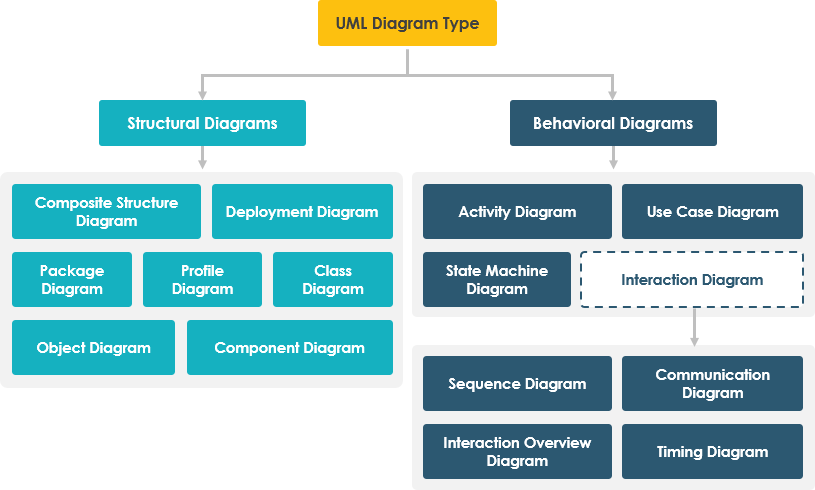
\includegraphics[width=1.0\linewidth]{01-uml-diagram-types.png}
    \caption{A map of the 14 UML diagram types, grouped into their respective categories, with an additional breakdown of the interaction diagrams subcategory\cite{visualpara}.}
    \label{fig:UML Diagram Map}
\end{figure}

\subsubsubsection{Sequence Diagram}

Sequence diagrams belong to a sub-category of interaction diagrams, which includes communication, timing, and interaction overview diagrams\cite{Seidl_Scholz_Huemer_Kappel_Duffy_2014}.

Sequence diagrams model communication protocols between human and non-human entities. The horizontal axis represents the sequence of communication messages, while the vertical axis shows the timing of interactions. Each element in a sequence diagram is represented by a lifeline extending vertically, which may terminate if it is no longer required in the system. Messages are represented by arrows connecting elements at various stages of their lifecycle. 

Figure 2 presents a simplified sequence diagram that expands on the earlier analogy of a \texttt{Human} class, showcasing interactions between its \texttt{person} instances.

\begin{figure}[H]
    \centering
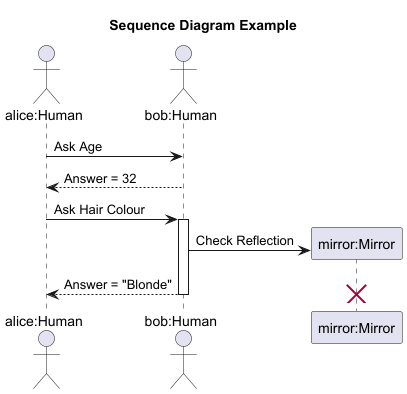
\includegraphics[width=0.7\linewidth]{SDexample-Sequence_Diagram_Example.png}
    \caption{A simple sequence diagram: Alice asks Bob his age and receives the reply "32". Bob consults a non-human "mirror" object to answer the second query, and the mirror's lifeline terminates once it is no longer needed.}
    \label{fig:enter-label}
\end{figure}

\subsubsubsection{Class Diagram}

The class diagram defines the structure of classes within a system\cite{Seidl_Scholz_Huemer_Kappel_Duffy_2014}. Each class is depicted as a rectangular element containing information about the attributes it holds and the operations it can perform. Interconnected edges represent the associations between different classes in the system, defining their specific relationships and interactions. The class diagram provides an overview of the modelled system's structural architecture. Figure 3 continues with the \texttt{Human} class analogy to give a simplified class diagram.

\begin{figure}[H]
    \centering
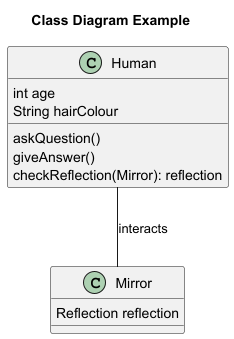
\includegraphics[width=0.4\linewidth]{CDexample-Class_Diagram_Example.png}
    \caption{A simple class diagram: The \texttt{Human} class has attributes \texttt{age} and \texttt{hairColour} and can perform the operations \texttt{askQuestion()}, \texttt{giveAnswer()}, and \texttt{checkReflection()} if given a mirror. It has an "interacts" association with a \texttt{Mirror} class, which returns its \texttt{reflection} attribute when \texttt{checkReflection()} is called.}
    \end{figure}

\subsubsubsection{Profile Diagram}

The profile diagram is another structural diagram used to modify general-purpose UML diagrams to become domain-specific.

The composition of a UML diagram is modelled using UML itself. Class diagrams illustrate the structure of each of the 14 UML diagram types, including their own structure. Together, these class diagrams form the UML meta-model\cite{Seidl_Scholz_Huemer_Kappel_Duffy_2014}.

There are three methods for tailoring the UML meta-model to a specific domain, with the appropriate approach chosen based on the required level of specificity. These methods, in order of decreasing intensity, are creating an entirely new meta-model for the domain, modifying the existing UML meta-model by introducing new meta-classes and meta-associations or leveraging UML's built-in extension mechanism—the UML profile diagram\cite{Seidl_Scholz_Huemer_Kappel_Duffy_2014}.

The profile diagram uses stereotypes, a type of meta-class, to modify existing meta-classes in the meta-model. For example, the meta-classes \textbf{Association} and \textbf{Class} are part of the class diagram meta-model, while \textbf{Message} and \textbf{Lifeline} are used in the sequence diagram meta-model. Stereotypes are denoted by the tag \texttt{<<Stereotype>>}, followed by their name. These stereotypes are connected to the meta-classes they modify through an extension relationship pointing from the stereotype to the meta-class it's modifying\cite{Seidl_Scholz_Huemer_Kappel_Duffy_2014}.

A stereotype can include meta-attributes or carry a note. Notes typically provide additional context or clarification in natural language. The stereotype name, meta-attributes, and notes impose constraints on the meta-class being extended, thus refining the system's structure and behaviour by introducing domain-specific constraints\cite{Seidl_Scholz_Huemer_Kappel_Duffy_2014}. 

Figure 4 illustrates how the profile diagram constrains the class diagram meta-model by applying stereotypes to its meta-classes. Figure 5 demonstrates how the class diagram is constructed using the stereotypes defined in Figure 4.

\begin{figure}[H]
    \centering
    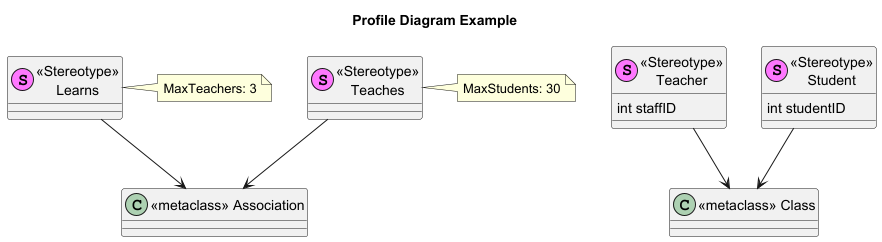
\includegraphics[width=1\linewidth]{PDExample-Profile_Diagram_Example.png}
    \caption{A simple profile diagram applied to the class diagram meta-model. The stereotypes \texttt{<<Teacher>>} and \texttt{<<Student>>} are applied to classes, each containing meta-attributes related to their respective IDs. The stereotypes \texttt{Learns} and \texttt{Teaches} are assigned to associations, with notes specifying limits on how many "teaches" or "learns" associations can exist within a system.}
\end{figure}

\begin{figure}[H]
    \centering
    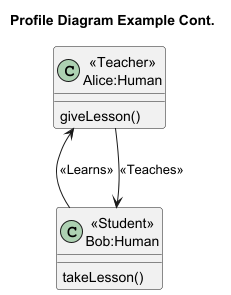
\includegraphics[width=0.3\linewidth]{PDExample2.png}
    \caption{A class diagram implementing the profile diagram stereotypes. Classes and associations are tagged with their respective stereotypes, inheriting the constraints defined in Figure 4.}
    \label{fig:enter-label}
\end{figure}

\subsubsection{Q-SE 2021}

The second Q-SE workshop held virtually in June 2021 included a segment focused on modelling quantum systems\cite{QSE2021}. During this session, Luis Jiménez-Navajas presented the paper \textit{"Modelling Quantum Circuits with UML"}\cite{Pérez-Castillo2021}, co-authored with Ricardo Pérez-Castillo and Mario Piattini. The paper introduced the concept of creating a UML profile diagram that could incorporate a quantum domain, using the example of an activity diagram to model a quantum circuit\cite{Pérez-Castillo2021}. 

Pérez-Castillo and Piattini further expanded on this work and, in 2022, published the paper \textit{"Design of Classical-Quantum Systems with UML"}\cite{Pérez-Castillo2022} in the Springer May 2022 \textit{Computing} journal\cite{Computing2022}. They also served as editors for \textit{“Quantum Software Engineering”}\cite{serrano2022quantum}, also published by Springer, which included a revision of Pérez-Delgado's Q-UML work. The follow-up paper, \textit{“A Quantum Software Modeling Language”}\cite{Pérez-Delgado2022}, further developed Q-UML by introducing additional pictorial elements for modelling quantum components and establishing fundamental axioms and core design principles.

\textit{"Design of Classical-Quantum Systems with UML"}\cite{Pérez-Castillo2022} built upon earlier efforts to develop a quantum UML profile diagram by extending its application to multiple UML diagram types. 

Pérez-Delgado's work with Q-UML modelled Shor's algorithm in the context of a quantum computer exhibiting quantum advantage, while Pérez-Castillo and Piattini modelled hybrid information systems. These hybrid systems, which combine classical and quantum processors, are already operational and can be executed on existing quantum hardware.

\subsubsection{NISQ}

As the introduction mentions, classical and quantum computers differ fundamentally in their underlying hardware. Classical computers operate in a binary, deterministic state where bits are clearly defined as 0 or 1. In contrast, quantum computers leverage the principles of quantum mechanics, using qubits instead of bits. A qubit can exist in a superposition of 0 and 1, with its final state determined probabilistically when measured. 

The ability for qubits to exist in superpositions allows quantum computers to accelerate the speed at which certain types of problems can be solved exponentially\cite{knowledgeacademy}. A well-known example is factoring large prime numbers, a computational task that classical computers find difficult to solve within a reasonable time frame. Peter Shor’s development of Shor’s algorithm demonstrates how a sufficiently powerful quantum computer could theoretically perform prime factorisation significantly faster than its classical counterpart\cite{Shor_1997}\cite{minutephysics}. The Rivest-Shamir-Adleman (RSA) encryption algorithm is a widely used encryption protocol which relies on classical computers' difficulty in factoring large prime numbers\cite{encryptionconsulting}. A powerful enough quantum computer could pose a risk to modern-day security protocols as we currently know them. 

Quantum computing aspires to reach the same level of ubiquity as classical computing while achieving quantum supremacy and quantum advantage. Quantum supremacy would enable quantum computers to solve tasks that classical computers cannot complete within a reasonable time frame, such as factorisation of large prime numbers\cite{quera}. Quantum advantage would allow quantum systems to solve real-world problems \textit{"faster than any classical algorithm running on any classical computer"}\cite{quera}. To reach this point, quantum computers must scale up the number of qubits required for complex calculations—a critical challenge they face today.

Qubits are susceptible to environmental decoherence and noise, which can lead to errors and affect their ability to retain their quantum state\cite{futurumcareers}. Despite notable progress in increasing qubit counts, significantly more qubits are needed to enable error-correction methods for fault-tolerant quantum computing required for quantum advantage and quantum supremacy.\cite{NewScientist}.

The Noisy Intermediate-Scale Quantum (NISQ) era, representing near-term quantum computing, refers to hardware with qubit counts ranging from tens to hundreds\cite{NISQ}. This technology is currently accessible, with IBM's Qiskit Runtime Service as an example of NISQ hardware utilisation\cite{ReleaseSummary}. Despite their limited qubit capacity, these systems support computations through hybrid algorithms that leverage quantum and classical resources. One such algorithm is the Variational Quantum Eigensolver, which enables practical problem-solving within NISQ constraints.

\subsubsection{VQE}

The Variational Quantum Eigensolver (VQE) is a hybrid quantum-classical algorithm that can be used to find the ground state, the lowest energy, of a given physical system\cite{wikivqe}. VQE can aid in quantum chemistry simulations where determining the ground state of a given molecule or atom \textit{"provides essential information about the system's stability, reactivity, and other chemical properties"}\cite{queragroundstate}. VQE has many potential applications but can be considered a viable candidate for optimisation problems; it can be used to find a global or best local minimum (or maximum) solution within a search space\cite{vqeqiskit}\cite{VQEMax}. 

VQE belongs to a class of near-term algorithms designed to run on NISQ devices. As the depth of a quantum circuit increases, error rates also rise due to decoherence, requiring more qubits for error correction. Near-term algorithms seek techniques for solving non-trivial problems using limited qubit count whilst negating decoherence\cite{Huang_2023}. VQE uses a shallow quantum circuit and delegates tasks between the quantum circuit and a classical optimiser to find its solution\cite{vqeqiskit}\cite{Peruzzo2014}.

The VQE algorithm contains the following core components:

\textbf{Hamiltonian} - A matrix that represents the total energy of a physical system\cite{hamiltonian}. The eigenvalues of the Hamiltonian correspond to the system's energy levels, with the lowest eigenvalue representing the system's ground state\cite{vqeqiskit}.

\textbf{Ansatz} - A trial state for the Hamiltonian that represents an educated guess for finding the Hamiltonian's approximate ground state. The ansatz is a parametrised quantum circuit, with its parameters iteratively updated and the energy estimate evaluated against the Hamiltonian to find the lowest energy estimate\cite{ansatz} \cite{wikiansatz} \cite{Tutorial}.

\textbf{Cost Function} - A function that defines the objective of the problem, whether it involves minimisation or maximisation. The cost function executes the parametrised ansatz quantum circuit to estimate the energy of the Hamiltonian\cite{Tutorial}\cite{vqeqiskit}.

\textbf{Optimiser} - A classical optimiser that evaluates the output of the cost function and iteratively adjusts the ansatz parameters, seeking to find the optimal set of parameters for the problem solution\cite{Tutorial}\cite{vqeqiskit}. 

The pseudocode for the VQE algorithm is as follows:

\begin{algorithm}[H]
\caption{Variational Quantum Eigensolver (VQE)}\label{vqe_algorithm}
\begin{algorithmic}[1]
\State Define Hamiltonian \( \mathcal{H} \)
\State Prepare ansatz \( \mathcal{A} \) with \( k \) parameters \( \overrightarrow{\theta} \)
\State Define cost function $\mathcal{C}$ as either minimisation ($\bigwedge$) or maximisation ($\bigvee$)
\State Initialise a classical optimizer \( O \)
\While{convergence criterion not met and max iterations not exceeded}
    \State Calculate expectation value \( E \) by evaluating \( \mathcal{A}(\overrightarrow{\theta}) \) with \( \mathcal{H} \)
    \State Update \( \overrightarrow{\theta} \) using \( O \) to optimise \( E \)
\EndWhile
\State \Return optimal parameters \( \overrightarrow{\theta} \) and solution \( E \)
\end{algorithmic}
\end{algorithm}

The VQE algorithm can be implemented and executed using quantum programming languages, with IBM’s Qiskit SDK being a popular choice.

\subsubsection{Qiskit}

Qiskit is an open-source software development kit (SDK) created by IBM to access and utilise their cloud-based quantum computing services. Written in Python, Qiskit provides tools and libraries for quantum programming, simulation, and experimentation.

IBM Quantum Learning offers online tutorials\cite{Tutorial} that guide users through implementing quantum algorithms with the Qiskit SDK. The UML diagrams created for this paper are based on the IBM tutorial demonstrating the VQE algorithm in Qiskit\cite{IBM2024}.

\subsubsubsection{Qiskit and VQE}

This section aims to provide the reader with a comprehensive overview of the specific implementation of VQE following the Qiskit IBM tutorial\cite{Tutorial}. The intention is to enable a thorough understanding of the associated UML diagrams. The code for this tutorial is provided in the appendix.

The instance \textbf{hamiltonian} is initialised from the class \textbf{SparsePauliOp} by calling the \textit{.from\_list()} method in its construction. The \textbf{hamiltonian} object is a classical representation of Pauli operators, where each operator is given as a string (e.g., "X", "Y", "Z", or "I" for identity). Pauli operators are 2×2 matrices corresponding to spin measurements along the x, y, and z axes\cite{DJORDJEVIC201229}. Each operator string specifies actions on individual qubits. The VQE tutorial uses a 2-qubit system, acting on pairs of Pauli strings referred to as operator terms. The tensor product of these pairs is assigned a coefficient (represented as a complex number in Python) that defines the strength of each operator term. The linear combination of these terms represents the system's total energy, the Hamiltonian. Only non-zero operators and coefficients are stored, resulting in a sparse representation of operator terms and the Hamiltonian as a whole to reduce computational expense\cite{EITCA2024}\cite{SparsePauliOp}\cite{PauliList}.

The instance \textbf{ansatz} is initialised from the class \textbf{EfficientSU2} with the number of qubits \textbf{hamiltonian} holds passed to it in its construction. The \textbf{EfficientSU2} class provides a hardware-efficient classical representation of a quantum circuit capable of creating parametrised quantum states\cite{ansatz}. The circuit comprises layers of single-qubit operations along with C-NOT gates, which entangle the qubits. The Qiskit documentation defines SU(2) as \textit{"the special unitary group of degree 2, its elements are 2×2 unitary matrices with determinant 1, such as the Pauli rotation gates"}\cite{EfficientSU2}, meaning that the circuit includes layers of operations that rotate the states of individual qubits, specifically using Pauli rotation gates. Each Pauli rotation gate holds a parameter which will be iteratively adjusted to find the lowest energy state of \textbf{ansatz}.

The instance \textbf{backend} is initialised from the class \textbf{QiskitRuntimeService}. The \textbf{QiskitRuntimeService} class interacts with the IBM Qiskit Runtime Service that provides cloud-based access to quantum hardware and quantum simulators. Creating an IBM account and giving a token when executing the code to access the service is necessary. The parameter \textbf{ibm\_quantum} is given to \textbf{backend} during its construction to access the quantum computing platform available on the IBM cloud service. The method \textit{least.busy()} is used to select the next available quantum hardware with the parameter \textbf{simulator} set to false to access the quantum hardware as opposed to a quantum simulator. 

\textbf{QiskitRuntimeService} will instantiate an \textbf{IBMBackend} object which interacts with the selected quantum hardware. The attribute \textbf{target} of the \textbf{IBMBackend} object is accessed and passed as a parameter to the instance \textbf{pm} of the \textbf{StagedPassManager} class, created using the \textit{generate\_preset\_pass\_manager()} method. This process allows the pass manager to receive information regarding the constraints of the selected quantum hardware.

The pass manager will \textit{"define a typical full compilation pipeline from an abstract virtual circuit to one that is optimized and capable of running on the specified backend"}\cite{StagedPassManager}. The \textit{.run()} method is executed on \textbf{pm} to transform \textbf{ansatz} to be compatible with the selected quantum hardware's instruction set architecture (ISA)\cite{IBM2024}, with the newly transformed ansatz stored in a new variable \textbf{ansatz\_isa}. The \textit{.apply\_layout()} method is then called on \textbf{hamiltonian}, with \textbf{ansatz\_isa} passed as a parameter, to modify its layout to be compatible with the selected quantum hardware ISA. The modified Hamiltonian is then stored as a new variable  \textbf{hamiltonian\_isa}.

A cost function method, defined as \textbf{cost\_func}, is a user-defined function that facilitates access to the quantum hardware and will obtain an approximate energy estimate of the Hamiltonian. It accepts an estimator and the components of a primitive unified bloc (PUB) as its parameters. 

 Qiskit offers two primary primitives—"Estimator" and "Sampler"—designed to simplify foundational quantum tasks\cite{QiskitRuntime}. Estimator primitives \textit{"accept combinations of circuits and observables (or sweeps thereof) to estimate expectation values of the observables"}\cite{Primitives}. The estimator accepts the quantum circuit \textbf{ansatz\_isa} and the Hamiltonian \textbf{hamiltonian\_isa} to produce an estimated expectation value of the Hamiltonian's energy. The estimator is defined later in the code, created by the class \textbf{EstimatorV2}. The PUB is the input given to the estimator primitive.

PUB comprises of an array of initial guesses for the parameters of the ansatz, the \textbf{hamiltonian\_isa} given as a list, and the quantum circuit \textbf{ansatz\_isa}. These components form a tuple and are assigned to the variable \textbf{pub}, which is given as a parameter for the estimator object's \textit{.run()} method. 

When \textit{estimator.run()} is executed, the classical, parametrised \textbf{ansatz\_isa} circuit is transpiled into a quantum circuit that is compatible with the selected quantum hardware. It is then executed on the quantum computer provided through the IBM cloud service, preparing a quantum state based on its current parameters\cite{EstimatorV2}\cite{Tutorial}. The \textbf{hamiltonian\_isa} list, which represents the system's Hamiltonian, is applied to this prepared quantum state. This guides the estimator in computing the energy expectation value of the system being modelled through the \textbf{ansatz\_isa} circuit. Once the operation is complete, the \textit{.result()} method returns a container of PUB results\cite{PrimitiveResult}, with slicing used to access the estimated energy of the \textbf{ansatz\_isa}, which is stored in the variable \textbf{energy}.

A dictionary named \textbf{cost\_history\_dict} stores the parameter, iteration, and energy estimate each time the estimator's \textit{.run()} method is executed. Its initial values consist of a placeholder for the parameters, iteration set to zero and an empty list for the energy estimate, with each energy estimate being appended to the list per execution. 

Finally, the cost function method returns the value of the \textbf{energy} variable as its result after being called.

A random array of initial guess parameters, assigned to the variable \textbf{x0}, is constructed using NumPy’s constant $\pi$ and its \textit{random.random()} method. The code generates an array of random floating-point numbers, scaled to the range of [0,$\pi$2], to account for every quantum state that can be represented on the Bloch sphere. The \textbf{ansatz} attribute \textbf{num\_parameters} sets the size of the array, having been stored earlier in the variable \textbf{num\_params}, to match the number of parameters to assign to each of the Pauli rotation gates in the ansatz circuit. The \textbf{x0} array will be given to \textbf{cost\_func} as the parameters required for the \textbf{pub} variable and updated iteratively to find the set of parameters that produce the lowest energy estimate of the system.

The instance \textbf{session} is initialised from the class \textbf{Session} with \textbf{backend} passed as a parameter to configure it to the selected quantum hardware. The instance \textbf{estimator} is then initialised from the class \textbf{EstimatorV2} with \textbf{session} passed to the estimator's \textbf{mode} attribute. This estimator, which operates within \textbf{cost\_func}, uses \textbf{session} to execute computations on the specified quantum backend. Assigning a  \textbf{Session} object as the estimator's \textbf{mode} facilitates the grouping of iterative calls to the quantum computer\cite{Session} when \textit{estimator.run()} executes, efficiently managing the allocation of jobs to quantum resources.

The instance \textbf{res} of the classical \textbf{Minimize} function from the SciPy package is initialised with the Constrained Optimization by Linear Approximation (COBYLA) method, which is used to minimise a scalar function\cite{Minimize}. In this case, the scalar function is the \textbf{cost\_func} method, which returns a scalar energy estimate as a float. The parameters for \textbf{res} include the \textbf{cost\_func}, the initial guess array \textbf{x0} for the ansatz parameters, along with \textbf{ansatz\_isa}, \textbf{hamiltonian\_isa}, and \textbf{estimator}, all passed from \textbf{res} to \textbf{cost\_func} for execution. 

During the optimisation loop, \textbf{cost\_func} calculates and returns the energy estimate of \textbf{ansatz\_isa}, while \textbf{res} iteratively updates the parameters in \textbf{x0}, adjusting the ansatz's parameters to minimize the energy estimate. Each call to \textbf{cost\_func} invokes the \textit{estimator.run()} method and performs 10,000 shots on the quantum circuit before returning the energy estimate. The loop continues until the energy estimate converges to the lowest achievable value, representing the ground-state energy\cite{Tutorial}.

Upon completion of the optimisation loop, successful termination of the process is verified by comparing the solution parameter and evaluation count against the stored solution parameter and iteration count within \textbf{cost\_history\_dict} maintained by the \textbf{cost\_func} method. These results are then visualised using the matplotlib package, plotting a graph with the number of iterations on the x-axis and the energy estimates on the y-axis.

\subsection{Related Work}

This section explores the two quantum adaptations to UML outlined in the Background. It summarises each paper's central argument and details the methodologies proposed for modifying UML or introducing extensions to accommodate quantum technology. These methodologies will be further examined and applied to the VQE algorithm, as detailed in the Design \& Implementation section.

\subsubsection{Q-UML}

The paper \textit{"A Quantum Software Modeling Language"} highlights the significant role modelling languages have played in enabling professionals from diverse disciplines to advance classical software engineering. This collaboration has been instrumental in making classical computers a ubiquitous part of modern life. Pérez-Delgado argues that while modelling large-scale quantum systems is not a pressing need, the introduction of a quantum modelling language could act as an \textit{intuition pump}, accelerating the development of quantum software engineering to achieve the maturity and integration of its classical counterpart\cite{Pérez-Delgado2022}.

Pérez-Delgado defines one fundamental axiom and five core design principles when constructing a quantum software modelling language. 

The fundamental axiom is that \textit{"quantum software
engineering should be as similar to classical software engineering as possible, but no more"}\cite{Pérez-Delgado2022}. A quantum modelling language must allow professionals familiar with classical software modelling techniques to adapt to its notation quickly. It must also clearly differentiate between its classical and quantum components as they handle fundamentally different types of information: \textit{"Quantum information can be put in superposition, classical information
cannot. Classical information can be cloned or copied, quantum information—in
general—cannot"}\cite{Pérez-Delgado2022}.

The five core design principles establish when and how classical and quantum elements must be differentiated in a quantum modelling language. They are explained as follows: 

\textbf{Quantum Classes}: If a class/object needs to use quantum information in its design or interactions, it must be labelled quantum.

\textbf{Quantum Elements}: Operations and attributes must be defined as either classical or quantum. The data types of variables must be labelled. The input and output of operations must be labelled. 

\textbf{Quantum Supremacy}: If an object does not use any quantum information for its design, interactions or relationships with other objects, it will always remain classical. It will be upgraded to quantum when it requires even one quantum element. 

\textbf{Quantum Aggregation}: An object composed of at least one other quantum object will be labelled as quantum.

\textbf{Quantum Communication}: Quantum and classical objects can communicate with each other if the message can be translated from quantum information to classical information. Quantum and classical messages must be labelled.

The axioms and design principles are culminated and applied to the UML extension Q-UML, with the paper providing examples of its implementation by example of a use case, class, state, activity, and sequence diagram modelling Shor's algorithm\cite{Pérez-Delgado2022}. Q-UML uses bold text and double lines to distinguish quantum elements in the diagram. Sections 3.4.1 and 3.5.1 delve deeper into the methodology for applying Q-UML to sequence and class diagrams.

\subsubsection{Quantum UML Profile}

The paper \textit{"Design of Classical-Quantum Systems with UML"} presents a quantum UML profile designed to address the gap in analysis and design techniques for hybrid classical-quantum information systems\cite{Pérez-Castillo2022}. 

Pérez-Castillo et al. highlights two main challenges in the development of quantum software practices: first, the ad-hoc approach to quantum programming languages, which is often \textit{"without any prior design or modelling"}\cite{Pérez-Castillo2022}, and second, the necessity for classical and quantum information systems to be \textit{"analysed and designed together"}\cite{Pérez-Castillo2022}. 

The authors argue that classical computers will not be replaced by quantum computers, as classical machines are still more cost-effective for many tasks. Instead, classical computers will serve as coordinators, managing requests to quantum software systems\cite{Pérez-Castillo2022}. This underscores the importance of developing design documentation that accommodates classical and quantum computing systems and outlines their interactions for design and analysis.

Pérez-Castillo et al. present UML as a viable tool for modelling hybrid quantum-classical systems. They reference Pérez-Delgado's Q-UML as an existing approach to modifying UML but classify it as a Domain-Specific Language (DSL) rather than a valid UML extension\cite{Pérez-Castillo2022}}. This distinction arises because Q-UML employs specific notations, such as double lines and bold text, which do not conform to the official UML standard. In contrast, the UML quantum profile diagrams outlined in the paper are considered UML-compliant, adhering to the existing UML specifications\cite{Pérez-Castillo2022}. 

Pérez-Castillo et al. introduce a UML profile for various UML diagram types, including use case, class, sequence, activity, and deployment diagrams. This paper will focus specifically on the class and sequence UML profile diagrams.

\subsubsubsection{Class Diagram Meta-Model}

The class diagram meta-model contains the stereotypes \texttt{<<Quantum>>}, \texttt{<<Quantum Driver>>}, and \texttt{<<Quantum Request>>}.

The \texttt{<<Quantum>>} stereotype constrains the meta-classes \textbf{Package} and \textbf{Class}. It is used to model classes and packages that enable quantum functionality such as \textit{"quantum
circuits, algorithms, or similar artefacts"}\cite{Pérez-Castillo2022}.

The \texttt{<<Quantum Driver>>} stereotype constrains the \textbf{Class} meta-class. It is used to model classes that manage communication with quantum software\cite{Pérez-Castillo2022}. 

The \texttt{<<Quantum Request>>} stereotype constrains the meta-classes \textbf{AssociationClass}, \textbf{Class}, \textbf{Dependency}, and \textbf{Operation}. It is an optional modelling choice used to represent calls from a \texttt{<<Quantum Driver>>} to a \texttt{<<Quantum>>} class, linking associated elements involved in the communication, such as cost functions and classical optimisers. It can also be used to model quantum operations within a class\cite{Pérez-Castillo2022}.

Figure 6 shows the class diagram meta-model with the application of the quantum UML profile extensions, as presented in the paper.

\begin{figure}
    \centering
    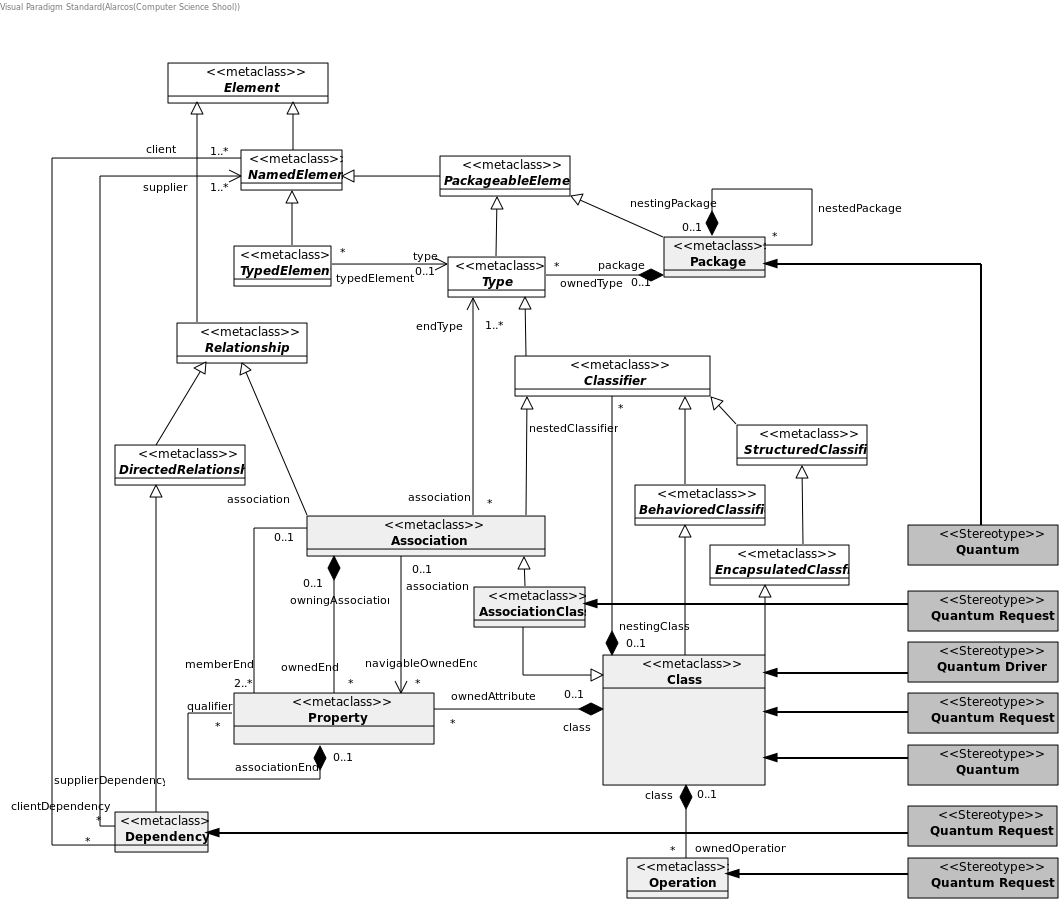
\includegraphics[width=1\linewidth]{QuantumUMLProfile-ClassDiagram.png}
    \caption{The quantum UML profile applied to the class diagram meta-model\cite{PerezCastillo2021Git}}
    \label{fig:enter-label}
\end{figure}

\subsubsubsection{Sequence Diagram Meta-Model}

The sequence diagram meta-model contains the stereotypes \texttt{<<Quantum Driver>>}, \texttt{<<Quantum>>}, \texttt{<<Quantum Request>>}, \texttt{<<Quantum Reply>>}, and \\ \texttt{<<Quantum Computer>>}.

The \texttt{<<Quantum Driver>>} and \texttt{<<Quantum>>} stereotypes both constrain the \textbf{Lifeline} meta-class. They align with the definitions established in the class diagram meta-model: \texttt{<<Quantum Driver>>} represents elements that enable communication with quantum software. The \texttt{<<Quantum>>} stereotype represents elements that provide quantum functionality.

The \texttt{<<Quantum Request>>} stereotype constrains the meta-class \textbf{Lifeline}, modelling elements created or linked by the call between a \texttt{<<Quantum Driver>>} and a \texttt{<<Quantum>>} element\cite{Pérez-Castillo2022}.

The \texttt{<<Quantum Request>>} and \texttt{<<Quantum Reply>>} stereotypes constrain the meta-class \textbf{Message}, modelling communications that either send or receive quantum information\cite{Pérez-Castillo2022}.

The \texttt{<<Quantum Computer>>} stereotype constrains the meta-class \textbf{Actor}, which denotes quantum machines if modelled in the diagram.

Figure 7 shows the sequence diagram meta-model with the application of the quantum UML profile extensions, as presented in the paper.

\begin{figure}
    \centering
    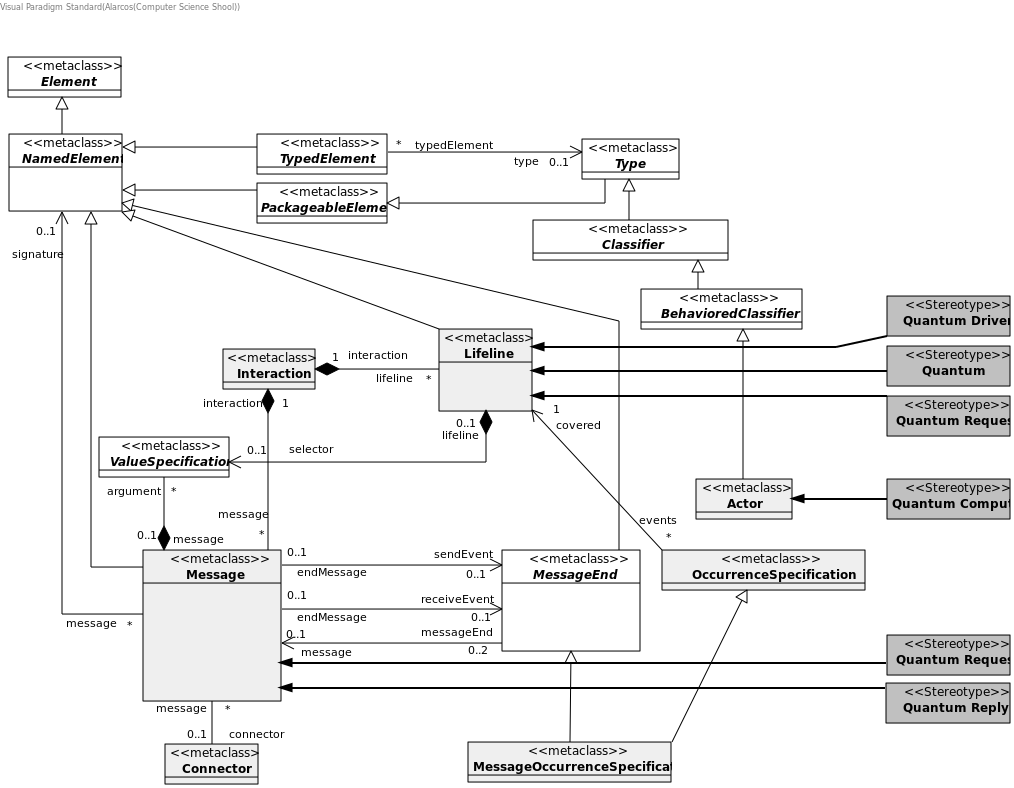
\includegraphics[width=1\linewidth]{QuantumUMLProfile-SequenceDiagram.png}
    \caption{The quantum UML profile applied to the sequence diagram meta-model\cite{PerezCastillo2021Git}}
    \label{fig:enter-label}
\end{figure}

\section{Design and Implementation}

This section details the creation of UML sequence and class diagrams used to model the VQE algorithm, as implemented on IBM's Quantum Learning platform. It begins with an overview of the tools employed for diagram creation, followed by a step-by-step breakdown of the diagram construction process. General notation conventions for all diagrams are outlined first, followed by a detailed explanation of how the VQE algorithm is represented in the sequence diagram. Subsequent sections explore how these diagrams are adapted into the Q-UML and quantum UML profile formats. The same approach is then applied to the VQE algorithm represented as a class diagram.

\subsection{Plant UML}

PlantUML is an open-source tool for creating various diagram types, including UML. It enables users to generate diagrams using plain text descriptions, which are then rendered into a graphical output\cite{PUML}\cite{PUMLWIKI}. The diagrams for this paper were initially drafted using the PlantUML plug-in for PyCharm.

\subsection{Lucidchart}

Lucidchart is a web-based application that supports creating a wide range of diagrams, including UML. It offers a user-friendly graphical interface for customisation and flexibility. To accommodate the Q-UML adaptations—such as the double-lined pictorial elements, which are not natively supported in PlantUML—the diagrams originally drafted in PlantUML were replicated in Lucidchart. This allowed for the necessary visual modifications and ensured consistency in comparison across both diagram adaptations.

\subsection{UML Design Choice}

UML offers users flexibility in choosing the level of detail required to represent system information within a diagram. It is essential to strike a balance between including sufficient information for clarity and avoiding over-complication, as UML diagrams should provide a high-level abstraction of the system. This section outlines the general formatting principles applied to all UML diagrams in this project. Subsequent sections on the VQE sequence and class diagrams will delve into specific design choices and their underlying rationale. Much of the reference material for constructing these diagrams has been sourced from the book UML @ Classroom\cite{Seidl_Scholz_Huemer_Kappel_Duffy_2014}. 

All UML diagrams consist of a content area populated by boxes and edges, which together form the specific design of each diagram type. An optional framing element was included in the UML diagrams for this project, enclosing these components within a boundary. The frame header displays the namespace of the system the diagram represents\cite{UMLElementFrame}. For this project, the namespace "Variational Quantum Eigensolver" is used, with abbreviations indicating the type of diagram preceding it. 

A sequence and class diagram have been created to model Qiskit’s implementation of the VQE algorithm. Additional versions of these diagrams have been adapted to illustrate the QUML and Quantum UML Profile extensions.

\subsection{VQE Sequence Diagram}

The elements in the sequence diagram represent instances of classes from Qiskit’s implementation of the VQE algorithm. Each instance is depicted as a rectangle, with a dashed, vertical lifeline extending downward from its creation to connect to a duplicated element at the bottom of the frame, where all the system elements are aligned. The naming convention follows the format \textit{instance:Class}.

Message sequences are simplified where possible to illustrate the provision of an attribute from one instance to another or to illustrate an operation's execution. For example, the message \textit{.num\_qubits} passed from the \textbf{hamiltonian} to the \textbf{ansatz} could have been a sequence of messages where the \textbf{ansatz} first requests the \textbf{.num\_qubits} attribute from the \textbf{hamiltonian} and the \textbf{hamiltonian} provides it as a response message, depicted by a dashed line and open arrowhead. This is more accurate; however, it would result in an over-complicated diagram of many messages. 

All messages in the diagram are synchronous, pointing from a sender to a receiver. A synchronous message indicates that the message must be received before the sender can continue with any further instructions\cite{Seidl_Scholz_Huemer_Kappel_Duffy_2014}. For example, the instance \textbf{pm:PassManager} cannot execute its \textit{pm.run(ansatz)} message until \textbf{backend:QiskitRuntimeService} passes its constraints and optimisation level. A continuous line and a filled triangular arrowhead depict a synchronous message.

A decision was made to omit the creation of an explicit \textbf{IBMBackend} element in the sequence diagram, opting instead to show messages invoking this object as originating from \textbf{backend:QiskitRuntimeService}.
The naming convention effectively conveys that \textbf{QiskitRuntimeService} serves as a "backend" instance. Adding \textbf{IBMBackend} would introduce unnecessary complexity to the sequence diagram, where the emphasis is on message flow rather than object details. These specifics are more appropriately captured in the class diagram, where \textbf{IBMBackend} has been included.

The transformation of \textbf{hamiltonian} and \textbf{ansatz} to \textbf{hamiltonian\_isa} and \textbf{ansatz\_isa} is depicted by a destruction event; a red cross on the lifeline at the point where \textbf{hamiltonian} and \textbf{ansatz} are no longer used in the system.

Activation bars depict the activation of multiple elements within the diagram when an operation is executed\cite{creatley}. This occurs when the pass manager executes its \textit{run.()} method, the  \textbf{hamiltonian} executes \textit{apply\_layout(layout=ansatz\_isa.layout)} and the execution of both \textbf{cost\_func} and \textbf{res}. Multiple elements within the system must be active to execute these operations.

The diagram uses two \textit{loop} fragments and an \textit{alt} fragment. The loop fragment expresses a sequence that is repeatedly executed\cite{Seidl_Scholz_Huemer_Kappel_Duffy_2014} with a boundary encompassing the messages involved in the repeated sequence. In the VQE sequence diagram, an outer loop fragment depicts the repeated exchange of messages between \textbf{cost\_func} and \textbf{res} as they seek to find the lowest energy estimate. An inner loop fragment depicts the repeated runs of the quantum circuit when \textit{estimator.run()} is executed. The upper right corner of the fragment contains a heading of the fragments label and a description of how long the process executes; the outer loop running until \textbf{[lowest energy estimate found]} and the inner loop running \textbf{[10,000 shots]}. The response message from the estimator is shown outside of this loop, as it does not return a result after each shot but once the circuit has completed 10,000 shots. 

The alt fragment in UML represents alternative sequences\cite{Seidl_Scholz_Huemer_Kappel_Duffy_2014}. Here, it evaluates whether the results of the \textbf{cost\_history\_dict} match those from the completed minimisation routine. A true or false boolean outcome determines whether the verification is successful or unsuccessful.

\subsubsection{SD QUML}

The elements \textbf{backend}, \textbf{res}, \textbf{estimator} and \textbf{cost\_func} are depicted as quantum through the use of bold text for their names, double lines for their rectangle elements and double lines for their lifelines. 

The instance \textbf{backend} facilitates communication between quantum and classical machines. Although the messages it sends in the diagram remain classical, the design of the class from which it is called, \textbf{QiskitRuntimeService}, is fundamentally quantum, following the first design principle \textbf{Quantum Classes}. The \textbf{estimator} element is also the instance of a quantum class that executes the ansatz circuit through its \textit{.run()} operation. The \textbf{cost\_func} element contains \textbf{estimator} in its design and is a user-define class in the context of this model. It, therefore, also follows the first design principle. The \textbf{res} element is a classical object that must be passed the \textbf{cost\_func} as parameters for its execution. As it contains at least one quantum element, it is upgraded to a quantum label, following the third design principle \textbf{Quantum Supremacy}. 

The sequence diagram includes one quantum message: \textbf{cost\_func} sends a request to \textbf{estimator} invoking its \textit{.run()} method on the PUB object at that iteration. This request triggers \textbf{estimator} to access quantum hardware and compute the energy estimate using quantum information based on the current parameters. The quantum nature of this message is denoted using double lines for the synchronous message, with the message details displayed in bold text. The reply message from \textbf{estimator} remains classical as the results are converted to classical information before being returned to \textbf{cost\_func}.

The corresponding diagram is presented in Figure 8.

\begin{sidewaysfigure}
    \centering
    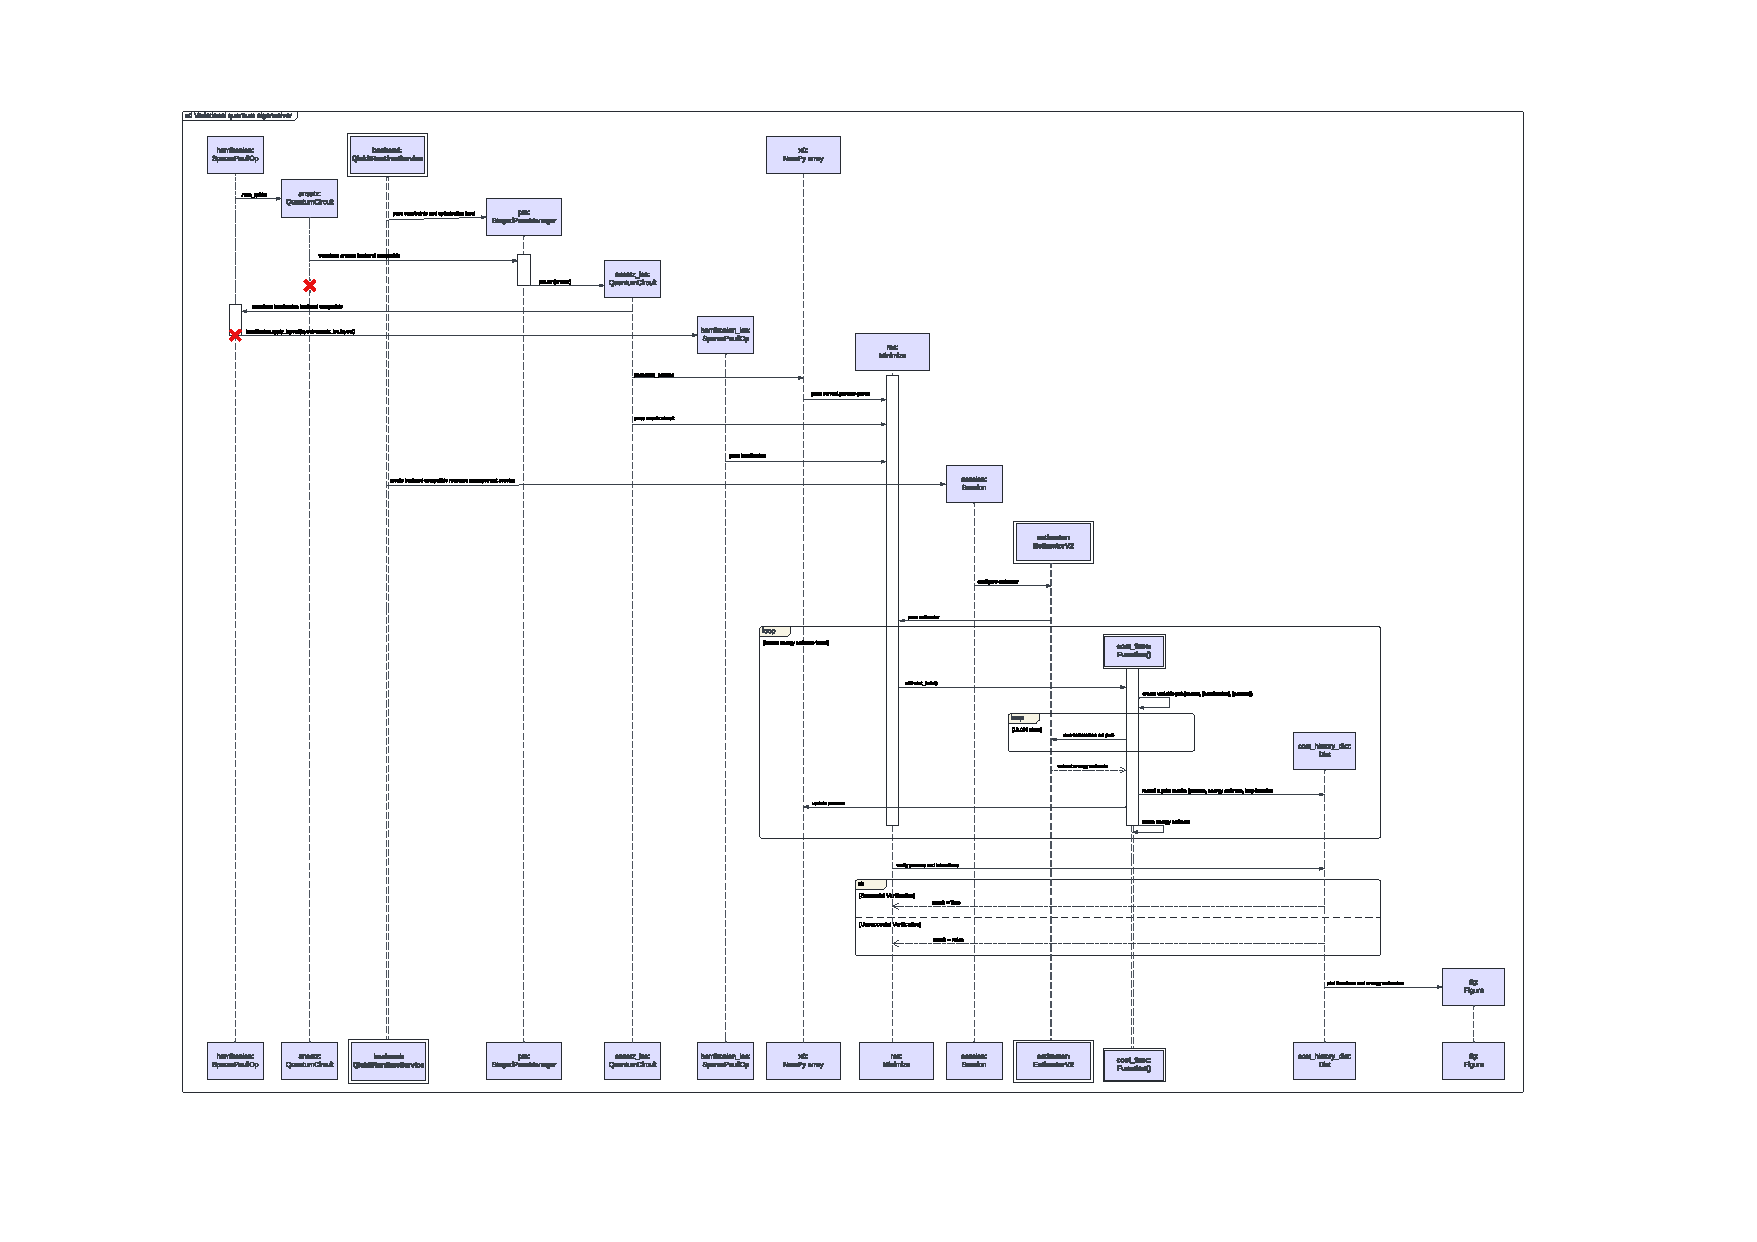
\includegraphics[width=1\linewidth]{VQE QUML SD Final Version.pdf}
    \caption{The application of Q-UML to a sequence diagram modelling the IBM Quantum Learning VQE Algorithm.}
    \label{fig:enter-label}
\end{sidewaysfigure}

\subsubsection{SD Quantum UML Profile}

The \textbf{backend} element, responsible for facilitating communication with quantum software, is assigned the stereotype \texttt{<<Quantum Driver>>}.

The \textbf{estimator} element, whose functionality executes quantum circuits, is assigned the stereotype \texttt{<<Quantum>>}.

The \textbf{cost\_func} element is directly tied to the interaction where a \texttt{<<Quantum Driver>>} invokes the \texttt{<<Quantum>>} element. It includes the operation \textit{estimator.run()} to execute this call, making it appropriate to assign the stereotype \texttt{<<Quantum Request>>}. The classical optimiser, \textbf{res}, is involved in this process but does not directly call \textit{estimator.run()}. Instead, it uses the classical output from \textbf{cost\_func} and provides classical input back to it. As its interactions remain classical, \textbf{res} is not assigned a quantum stereotype.

Similarly to Q-UML, the message from \textbf{cost\_func} calling the estimator's \textit{.run()} method is assigned the \texttt{<<Quantum Request>>} stereotype as it is a message containing quantum information. There is no \texttt{<<Quantum Reply>>} stereotype as the estimator converts the message back into classical information before being received by \textbf{cost\_func}.

The corresponding diagram is presented in Figure 9.

\begin{sidewaysfigure}
    \centering
    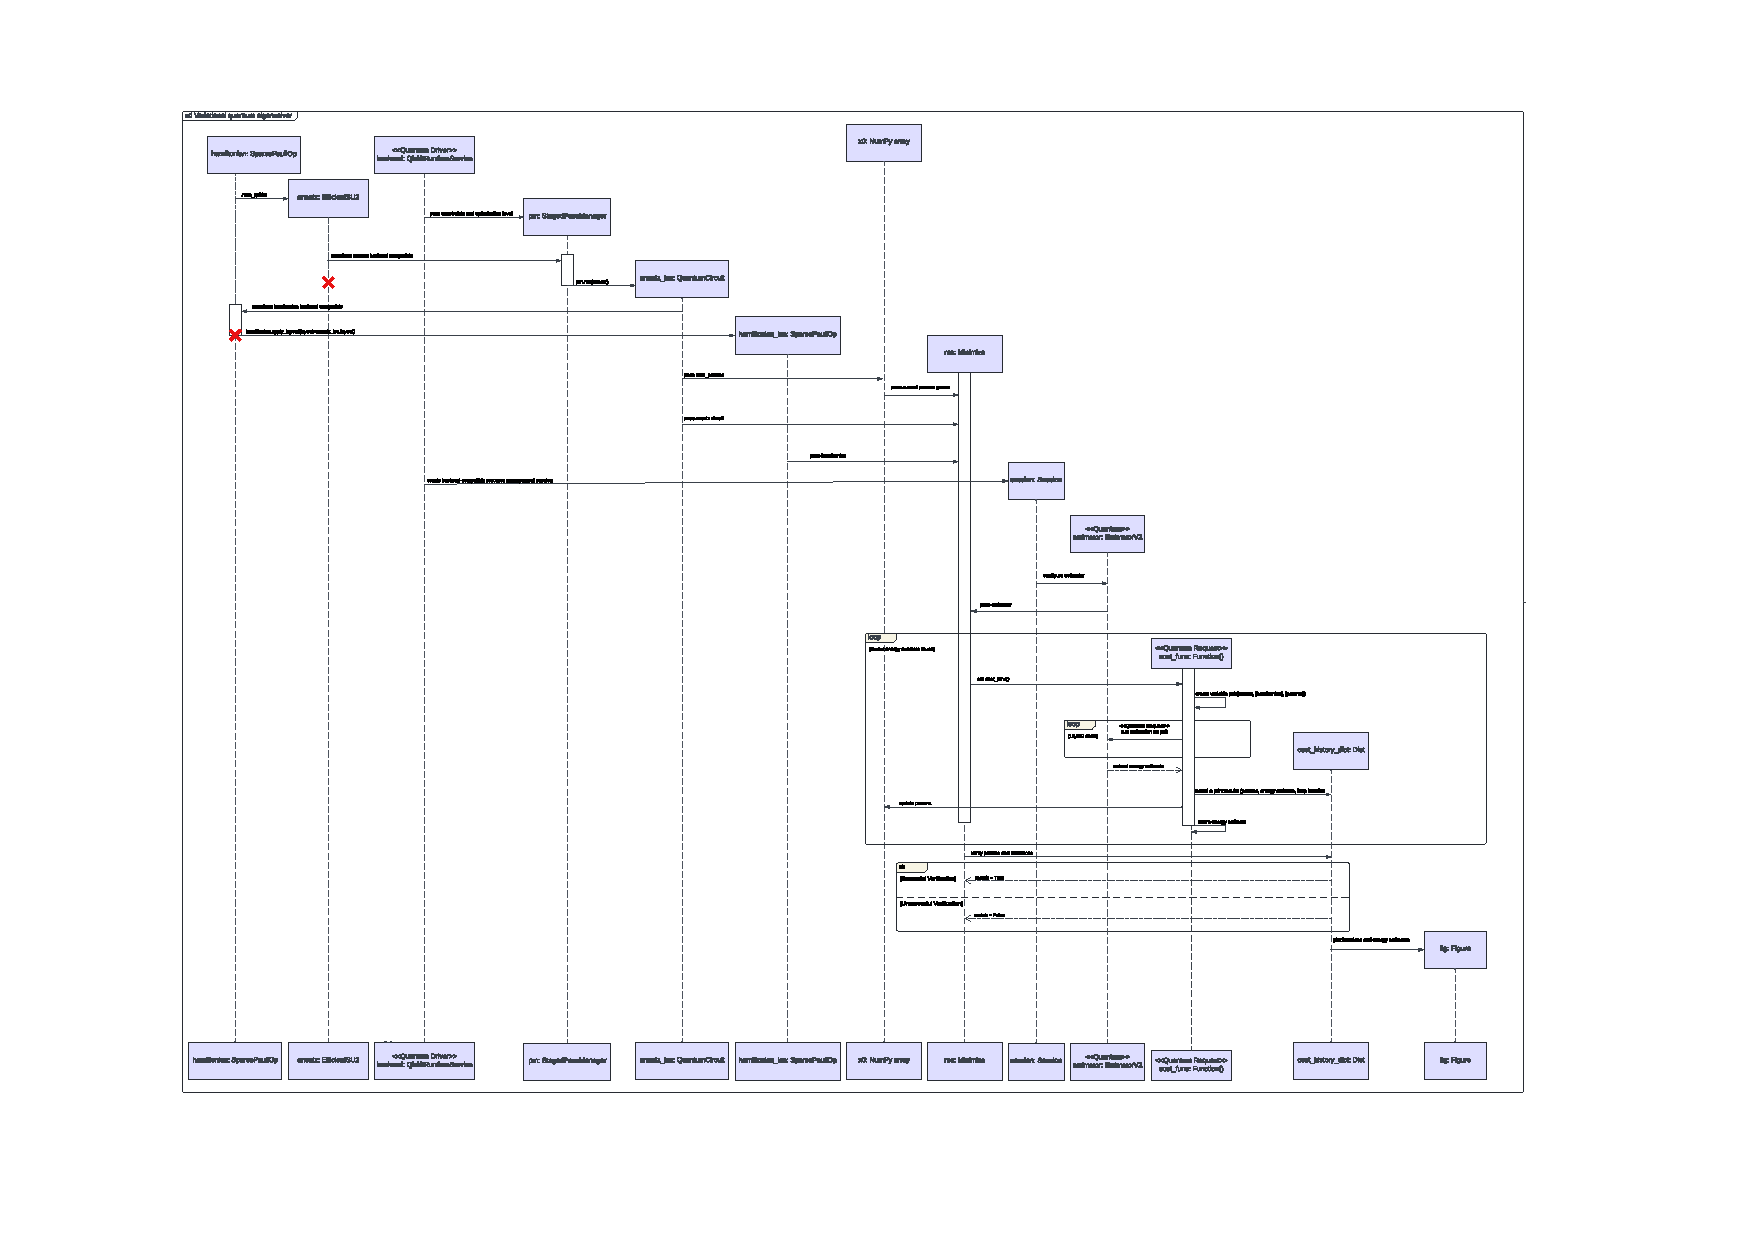
\includegraphics[width=1\linewidth]{VQE UML Profile SD Final Version.pdf}
    \caption{The application of the quantum UML profile to a sequence diagram modelling the IBM Quantum Learning VQE Algorithm.}
    \label{fig:enter-label}
\end{sidewaysfigure}

\subsection{VQE Class Diagram}

Packages group the imported Python libraries used to execute the VQE algorithm in Qiskit. Although the Qiskit SDK is more than a library, encompassing a collection of libraries alongside other utilities\cite{SheriefAbul-Ezz}, it is depicted as a single package for simplicity. Packages in UML are typically used for larger, more complex software systems\cite{VisualParadigm}; however, it was elected as a design choice to provide a clear visual of the required imports to run the algorithm. The design of a package element in UML resembles the structure of loop and alt fragments in sequence diagrams, grouping related elements within defined boundaries. However, unlike loop and alt fragments, which display their names in the upper-left corner inside the boundary, a package’s name appears in a smaller rectangle positioned outside of the boundary. The package \textbf{NumPy} is embedded within the Qiskit package—a design choice to prevent overlapping edges rather than imply a nested structure.

The class diagram elements, depicted as rectangles, illustrate the classes used in Qiskit’s VQE algorithm implementation, with each rectangle divided into three sections: namespace, attributes, and operations. A design choice was made to keep the same notation of \textit{instance:Class} for the namespace, as used in the sequence diagram. This notation is typically used in object diagrams. Class diagrams provide a static system view and typically only include the class name. In contrast, object diagrams capture the system at runtime and use either \textit{instance}, \textit{instance:Class} or \textit{:Class} as its naming convention\cite{Seidl_Scholz_Huemer_Kappel_Duffy_2014}. The decision to retain the instance in the notation is for clarity's sake, providing a minimal but effective indication of which class represents what aspect of the VQE algorithm by the instance name. Without an in-depth knowledge of Qiskit, it may be difficult to determine that \textbf{EfficentSU2} represents the ansatz or \textbf{SparsePauliOp} represents the Hamiltonian.

A design choice was also made to create a separate diagram for the \textbf{Minimize} class, distinct from the \textbf{CostFunction} class. Attempts to depict all class connections in a single diagram led to overlapping edges and clutter. The resulting diagram remains clear and readable by isolating \textbf{Minimize} and connecting it with simplified classes from the Qiskit package. The simplified classes are enclosed within the Qiskit package to indicate the part of the system to which they belong. The only simplified class not included is \textbf{CostFunction}, as it caused visual alignment issues. Since \textbf{CostFunction} is a user-defined method rather than a Qiskit class, it was decided to keep it outside the package in the minor diagram. Its meaning should still be evident within the complete diagram's context.

Only the attributes and methods relevant to the VQE algorithm are shown; additional attributes and methods documented in these classes have been omitted for clarity.

Some elements in the diagram, such as \textbf{Numpy.ndarray}, \textbf{CostFunction}, and \textbf{Dict}, are user-defined classes and therefore lack documentation detailing their attributes and operations. The variables and methods within these objects are presented directly as the attributes and operations of these elements in the diagram.

Each class attribute and method contains a visibility marker and it's name with the format "visbility\textbf{name:}". The visibility of all attributes and methods within the system is public, distinguished by the character +, meaning they are accessible to all other objects within the system\cite{Seidl_Scholz_Huemer_Kappel_Duffy_2014}. This was determined by none of the attributes or methods containing a leading underscore, which is the convention used in Python to define private attributes and methods\cite{Privacy}.

Class attributes contain their datatype with the format "visbility\textbf{name:} data type". Some class attributes also include multiplicities, which can be seen in the classes \textbf{SparsePauliOp}, \textbf{EfficientSU2}, \textbf{QiskitRuntimeService}, \textbf{EstimatorV2}, \textbf{Dict}, and \textbf{Pyplot}. Attribute multiplities are used in these classes to convey how many values the attribute can hold\cite{Seidl_Scholz_Huemer_Kappel_Duffy_2014}, with [0...1] indicating either none or one value or [1...*] to indicate one or many values. Attributes where multiplicities are omitted are considered to have only one value. Attributes with multiplicities also have additional information as to whether the values can be duplicated with the terms "unique" or "non-unique" and whether the values must be in a fixed order with the terms "ordered" or "unordered"\cite{Seidl_Scholz_Huemer_Kappel_Duffy_2014}. The format for an attribute which contains all of these details is "visbility\textbf{name:} data type[multiplicity]\{duplication,order\}". When an attribute's data type is a tuple, such as the \textbf{pub} attribute in \textbf{CostFunction}, each item's name and data type are specified, with square brackets enclosing the entire tuple to indicate its structure. Attributes can contain multiple data types. For example, the \textbf{mode} attribute of \textbf{Estimatorv2} can be assigned other data types than just Session. The name of the data type used in the specific algorithm is used for clarity. Including attributes is optional, with some classes not requiring this information, such as \textbf{StagedPassManager} and \textbf{Session}. 

Class methods are shown with either empty parentheses if no parameter information is needed or with detailed parameter information listed within the parentheses. The data type of the returned value is provided after the parentheses. The typical notation for a method with parameter information is "visbility\textbf{name}(\textbf{parameter name:} parameter data type): returned data type. For methods returning tuples—such as the \textit{from\_list()} method in \textbf{SparsePauliOp}, the \textit{run()} method in \textbf{Estimator}, and the \textit{res()} method in \textbf{Minimize}—each item's name and data type are specified and enclosed in square brackets, mirroring the method's format in code. 
The methods \textit{plot()}, \textit{set\_xlabel()}, and \textit{set\_ylabel()} in the \textbf{Pyplot} class do not have a return data type, as they do not return a value. Instead, they update a Figure object by assigning relevant information. The final output, of type Figure, is produced when the \textit{draw()} method is executed. Some classes, like \textbf{CostFunction} and \textbf{Minimize}, are methods themselves. These classes include methods with the class instance name, indicating that the class can be executed as an operation. Including operations is optional, with some classes not requiring this information, such as \textbf{IBMBackend} and \textbf{Dict}. 

Relationships, known as associations, between classes, are depicted by the edges that join the rectangles of the diagram. Edges with a solid line and filled triangular arrowhead pointing from one class to another indicate a binary association, where one class can view the visible attributes and operations of another class, but not the other way round\cite{Seidl_Scholz_Huemer_Kappel_Duffy_2014}. For example, \textbf{Session} can view the attributes and operations of \textbf{QiskitRuntimeService}, but \textbf{QiskitRuntimeService} cannot view the attributes and operations of \textbf{Session}. The edges between \textbf{SparsePauliOp} and \textbf{EfficentSU2} do not have arrowheads, meaning they are bidirectional\cite{Seidl_Scholz_Huemer_Kappel_Duffy_2014}; each class can view the other's attributes and operations. As we established earlier, all attributes and operations in the system are public and can technically be accessed by all objects. In the context of the VQE algorithm, the associations indicate which objects share and which objects receive information. Specifically, \textbf{SparsePauliOp} and \textbf{EfficientSU2} provide each other with information throughout the VQE algorithm. In contrast, \textbf{QiskitRuntimeService} provides information to \textbf{Session}, but \textbf{Session} does not provide information to \textbf{QiskitRuntimeService}.

The \textbf{IBMBackend} class depends on the \textbf{QiskitRuntimeService} class. This is depicted by a dashed line with an open arrowhead pointing from the dependent object to the object it depends on. The Qiskit documentation states that IBMBackend must not be instantiated directly and instead should be interacted with using the methods in \textbf{QiskitRuntimeService}\cite{IBMBackend}. The \textbf{IBMBackend} class is included in this diagram as its documentation contains the \textbf{target} attribute, which must be passed to \textbf{StagedPassManager} to access information regarding the selected quantum hardware constraints. The relationship has the stereotype \texttt{<<instantiate>>} as \textbf{IBMBackend} requires \textbf{QiskitRuntimeService} for it's full implementation\cite{Dependencyrelationships}

The class \textbf{Dict} is a composition of the class \textbf{CostFunction}. A composition is a binary association signifying that one class is contained as part of another class and cannot exist without it; if the aggregate(whole) object is destroyed, the contained part is also destroyed\cite{UMLComposition}. The relationship is depicted on the association edge by a filled diamond attached to the aggregate class. In this case, \textbf{Dict} is an integral part of \textbf{CostFunction} as it's written inside the method, remembering that the class \textbf{CostFunction} represents a user-defined method. If \textbf{CostFunction} were destroyed, \textbf{Dict} would also be destroyed.

Shared aggregation is similar to composition in that it signifies that one class belongs to another\cite{Seidl_Scholz_Huemer_Kappel_Duffy_2014}. However, unlike a composition, the contained classes can exist outside the aggregated class. A hollow diamond attached to the aggregate class depicts the relationship on the association edge. Shared aggregation is used to describe classes that are passed as parameters to other classes in the VQE algorithm; \textbf{Numpy:ndarray}, \textbf{EfficentSU2}, \textbf{EstimatorV2}, and \textbf{SparsePauliOp} are all passed as parameters to \textbf{CostFunction} and therefore have shared aggregation. The classes along with \textbf{CostFunction} are also passed to \textbf{Minimize} as parameters and, therefore, have shared aggregation. 

Some associations may be given an association name with a reading direction indicated by a filled triangular arrowhead pointing from one class to another. This arrowhead signifies the flow of the association's action, helping to clarify the direction in which information or control is passed between the classes involved. For example, the association between \textbf{StagedPassManager} and \textbf{EfficientSU2} shows that the pass manager will transform the ansatz and not the other way around. Although the reading direction points in the same direction as the binary association in this example, it does not have to\cite{Seidl_Scholz_Huemer_Kappel_Duffy_2014}.

The relationships between the classes in the diagram are defined by multiplicities, which specify how many objects are involved in each association. For instance, the binary association between \textbf{StagedPassManager} and \textbf{EfficientSU2} demonstrates that one instance of \textbf{StagedPassManager} is associated with exactly one instance of \textbf{EfficientSU2}. Multiplicities in the diagram are either \textbf{1} or \textbf{1..*}, with the option to label shared attributes. In the case of the \textbf{Minimize} class, it shares between one and many values of the attribute \textbf{res.x}—which contains parameters it iteratively updates—with a single \textbf{Numpy.ndarray} object. Subsequently, \textbf{Numpy.ndarray} shares only one array object with \textbf{CostFunction}. The use of multiplicities conveys a single-instance relationship between \textbf{Numpy.ndarray} and \textbf{CostFunction} while showing that \textbf{Minimize} dynamically updates and shares multiple values of \textbf{res.x} to the \textbf{Numpy.ndarray} class.

\subsubsection{CD QUML}

The classes \textbf{CostFunction}, \textbf{QiskitRuntimeService}, \textbf{IBMBackend}, \textbf{EstimatorV2}, and \textbf{Minimize} are depicted as quantum through the use of bold text for their names and double lines for their rectangles. This remains consistent with the sequence diagram quantum object labelling, with the inclusion of \textbf{IBMBackend} being a dependent object of \textbf{QiskitRuntimeService}.

No quantum attributes are shown, as all quantum data is translated into classical information for storage within these classes.

Quantum operations and input and output data types are highlighted in bold to indicate their quantum nature. The \textbf{QiskitRuntimeService} class includes two operations that return the class \textbf{IBMBackend} as a quantum data type. Similarly, the sole operation of the \textbf{Session} class also outputs an \textbf{IBMBackend} quantum data type. The \textbf{EstimatorV2} class features a quantum operation, \textit{.run()}, which interacts with quantum hardware and returns an object of the class \textbf{RuntimeJobV2}. While the returned information remains classical, \textbf{RuntimeJobV2} is intrinsically tied to a quantum communication process of extracting and translating quantum information as a classical output. Consequently, \textbf{RuntimeJobV2} is classified as a quantum data type in this context, similar to the depiction of \textbf{QiskitRuntimeService} as a quantum object in the sequence diagram. 

The \textbf{CostFunction} class contains itself as a quantum operation and produces a classical return value of type \textbf{numpy.float64}. Similarly, the \textbf{Minimize} class also contains itself as a quantum operation returning the classical data type \textbf{OptimizeResult}. The \textbf{Minimize} class includes parameters structured as a tuple, requiring the quantum input data type \textbf{EstimatorV2} to be provided.

A single quantum aggregation relationship exists between \textbf{EstimatorV2} and \textbf{CostFunction}, represented by a double-lined edge. In this relationship, the \textbf{EstimatorV2} quantum class is passed as a parameter to \textbf{CostFunction}.

The corresponding diagram is presented in Figure 10.

\begin{sidewaysfigure}
    \centering
    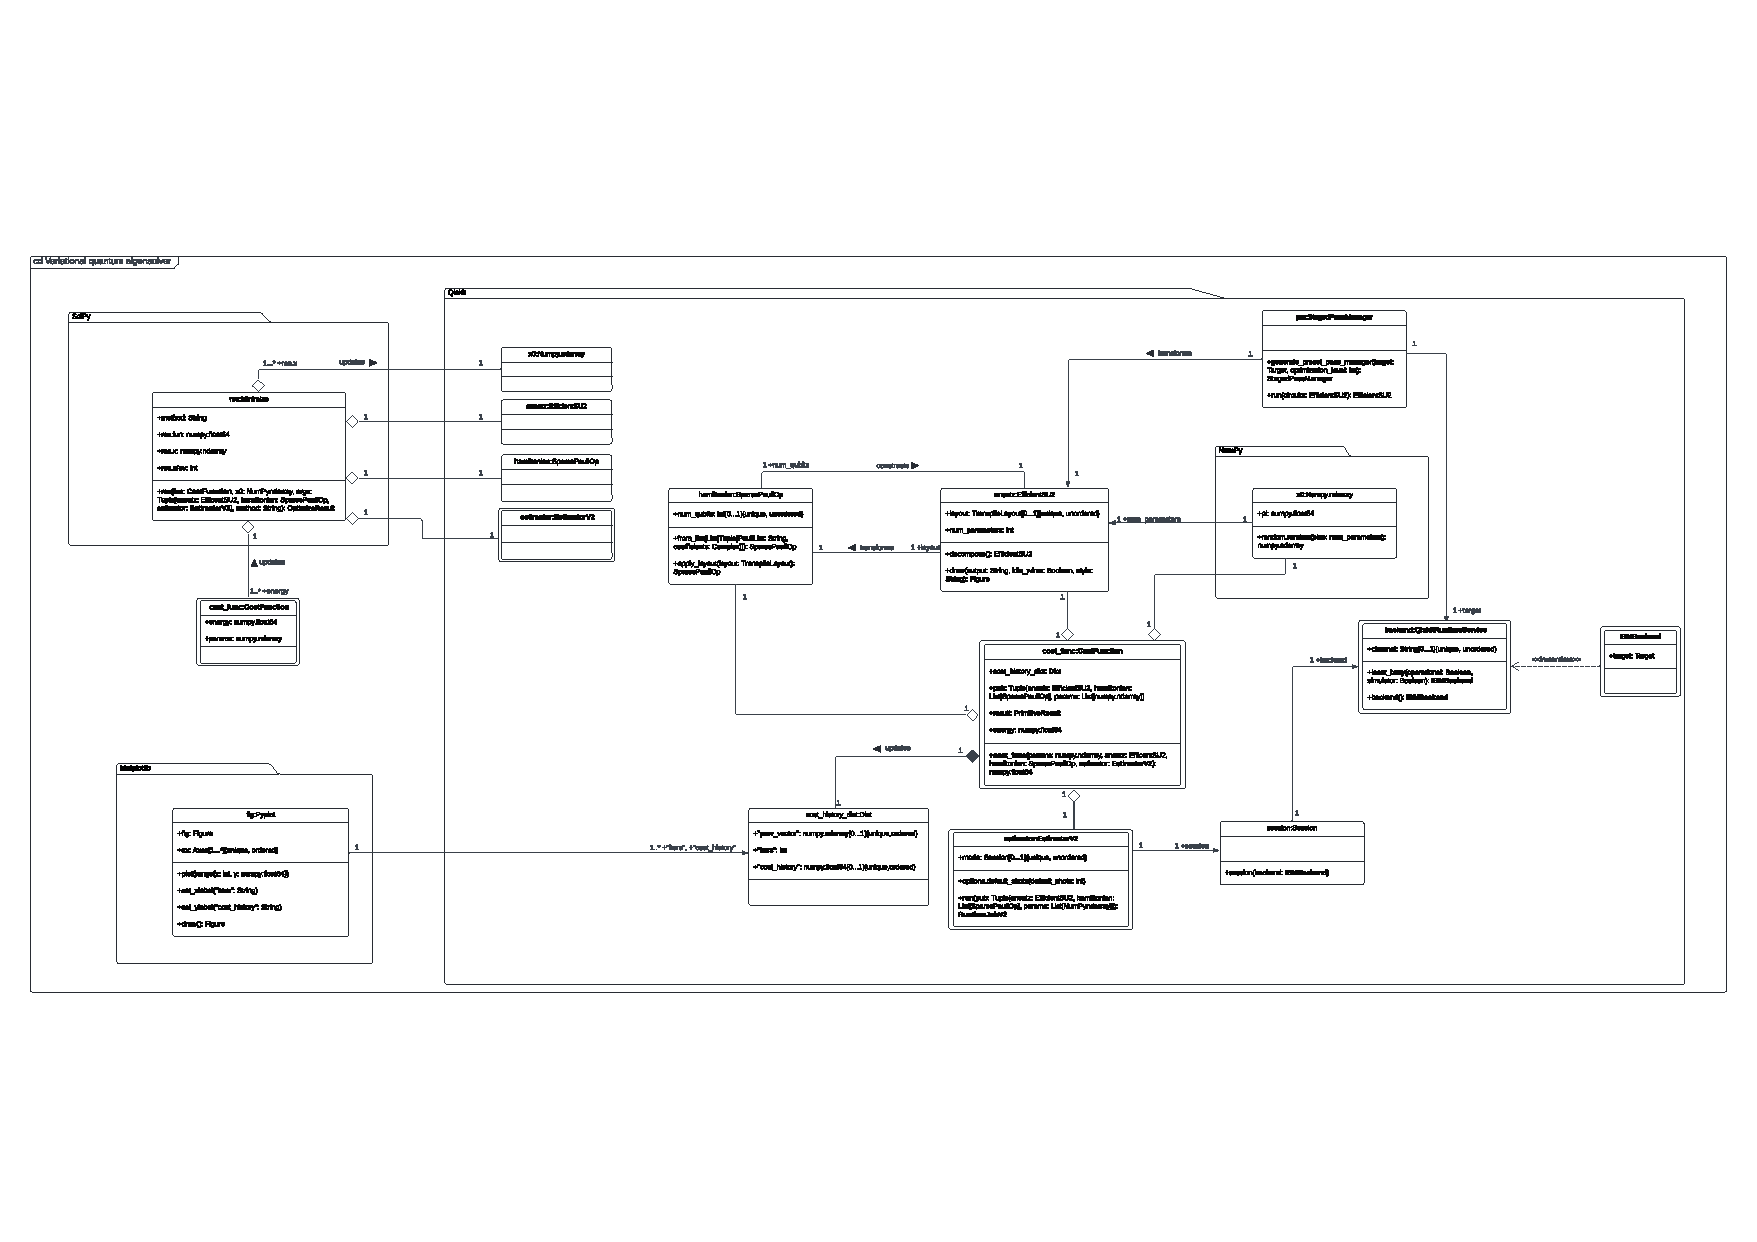
\includegraphics[width=1\linewidth]{VQE QUML CD Final Version.pdf}
    \caption{The application of Q-UML to a class diagram modelling the IBM Quantum Learning VQE Algorithm.}
    \label{fig:enter-label}
\end{sidewaysfigure}

\subsubsection{CD Quantum UML Profile}

The Qiskit package is assigned the stereotype \texttt{<<Quantum>} as it is a package that enables quantum functionality, allowing users to access quantum computers through the Qiskit SDK. 

The classes \textbf{CostFunction}, \textbf{EstimatorV2}, and \textbf{QiskitRuntimeService} inherit the same stereotypes as those assigned to their counterpart lifelines in the sequence diagram. Additionally, the \textbf{IBMBackend} class, which depends on \textbf{QiskitRuntimeService}, is assigned the \texttt{<<Quantum Request>>} stereotype. This assignment reflects its ability to perform the same quantum-related operations as the class on which it depends.

The operation \textit{.run()} in \textbf{EstimatorV2} and \textit{cost\_func()} in \textbf{CostFunction} are assigned the stereotype \texttt{<<Quantum Request>>}. Both operations are quantum as discussed previously; \textit{estimator.run()} invokes a call from the \texttt{<<Quantum Driver>>} to the \texttt{<<Quantum Element>>} and \textbf{CostFunction} contains this operation in it's design.

The corresponding diagram is presented in Figure 11.

\begin{sidewaysfigure}
    \centering
    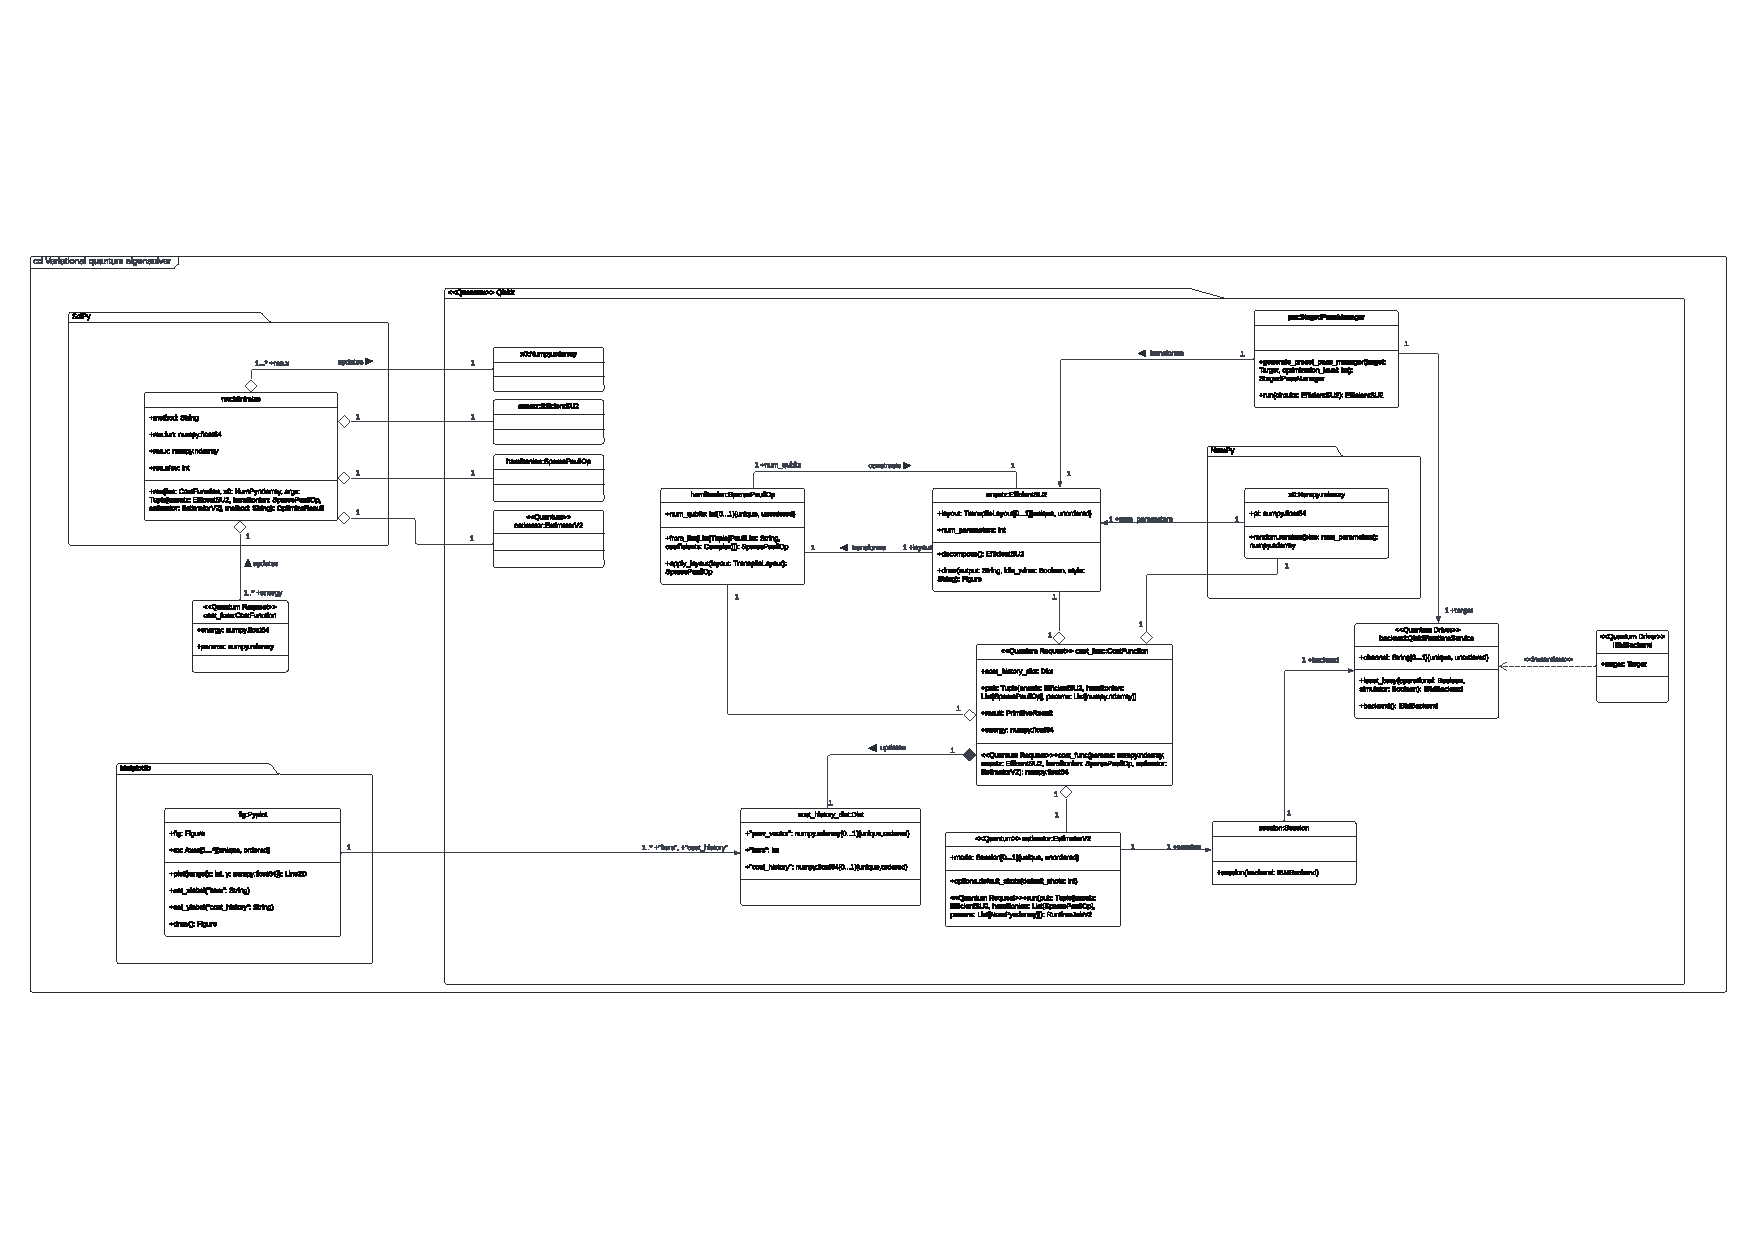
\includegraphics[width=1\linewidth]{VQE UML Profile CD Final Version.pdf}
    \caption{The application of the quantum UML profile to a class diagram modelling the IBM Quantum Learning VQE Algorithm.}
    \label{fig:enter-label}
\end{sidewaysfigure}

\section{Results and Analysis}

\subsection{Author Observations}

To create the Q-UML version of the VQE sequence diagram, a combination of Plant UML and Lucidchart was used to include the double lines and bold text necessary to distinguish quantum components. However, for creating the quantum UML profile, Plant UML alone may suffice, as it should have the tools required to extend UML to represent quantum-specific elements. 

The first completed diagram is a PNG file created in Lucidchart. An attempt was made to keep it to a format similar to the Plant UML output. Consistency must be considered to ensure a fair comparison between both diagrams; therefore, even if the VQE quantum UML profile diagram can be reproduced in Plant UML alone, it may need to be translated into Lucidchart to ensure this consistency is upheld.

My initial observations of the first diagram suggest that while the bold text and double lines used to distinguish quantum components are visible, they are more easily identifiable in examples provided in the Q-UML paper. This is likely due to the larger scope of the VQE sequence diagram and the fact that it is primarily composed of classical elements.
Additional design choices could be considered to better differentiate between classical and quantum components, although these would fall outside UML standards. For example, different colours could represent classical and quantum modules. This feature would only be readily available in applications like Lucidchart but could be incorporated with Plant UML by developing an extension.
Once the quantum UML profile version of the VQE sequence diagram is completed, more detailed observations and comparisons between the two diagrams will be possible.

\subsection{Diagram Literature}

Once both diagrams are completed, it will be crucial to consult relevant literature on effective diagram design to make an informed assessment. Research papers exploring good diagram design, particularly concerning UML, should be considered. An example of such work is the paper "Improving Information System Design: Using UML and Axiomatic Design" \cite{CAVIQUE2022103569}, which provides valuable insights into improving system information design.

\section{Conclusions}

The paper will conclude with an overall assessment of the advantages and disadvantages of each method. It will address whether the primary goal and all four main objectives were achieved. Additionally, there will be a discussion on whether UML is the most suitable approach for representing quantum systems or if a more general flowchart format might be more appropriate. This will include considering which method could be used in such a case. I assume that Q-UML would remain the most applicable, as the quantum UML profile is inherently based on UML formatting.

\section{Future Work}

Depending on whether the fourth objective is achieved, further exploration into modelling fundamental quantum concepts would be beneficial for evaluating the effectiveness of applying UML to quantum systems.
Plant UML is currently the most convenient tool for creating UML diagrams, as Lucidchart is significantly more labour-intensive. Developing an extension for Plant UML or other open-source tools like Mermaid to incorporate Q-UML formatting would be highly advantageous for future diagram creation. Such an extension would also increase the utility of this method, making it more accessible for continued exploration and broader adoption in the QSE field.

\printbibliography

\section{Appendix}

\subsection{IBM Quantum Learning VQE Code}

Below is the example code provided by IBM Quantum Learning to implement the VQE algorithm in Qiskit\cite{Tutorial}.

\begin{lstlisting}[language=Python]
# General imports
import numpy as np

# Pre-defined ansatz circuit and operator class for Hamiltonian
from qiskit.circuit.library import EfficientSU2
from qiskit.quantum_info import SparsePauliOp

# SciPy minimizer routine
from scipy.optimize import minimize

# Plotting functions
import matplotlib.pyplot as plt

# Runtime imports
from qiskit_ibm_runtime import QiskitRuntimeService, Session
from qiskit_ibm_runtime import EstimatorV2 as Estimator

# To run on hardware, select the backend with the fewest number of jobs in the queue
service = QiskitRuntimeService(channel="ibm_quantum")
backend = service.least_busy(operational=True, simulator=False)

# Define Hamiltonian
hamiltonian = SparsePauliOp.from_list(
    [("YZ", 0.3980), ("ZI", -0.3980), ("ZZ", -0.0113), ("XX", 0.1810)]
)

# Create ansatz
ansatz = EfficientSU2(hamiltonian.num_qubits)
num_params = ansatz.num_parameters

# Initalise pass manager
from qiskit.transpiler.preset_passmanagers import generate_preset_pass_manager

target = backend.target
pm = generate_preset_pass_manager(target=target, optimization_level=3)

# Transform ansatz
ansatz_isa = pm.run(ansatz)

# Transform Hamiltonian
hamiltonian_isa = hamiltonian.apply_layout(layout=ansatz_isa.layout)

# Define Cost Function
def cost_func(params, ansatz, hamiltonian, estimator):
    """Return estimate of energy from estimator

    Parameters:
        params (ndarray): Array of ansatz parameters
        ansatz (QuantumCircuit): Parameterized ansatz circuit
        hamiltonian (SparsePauliOp): Operator representation of Hamiltonian
        estimator (EstimatorV2): Estimator primitive instance
        cost_history_dict: Dictionary for storing intermediate results

    Returns:
        float: Energy estimate
    """
    pub = (ansatz, [hamiltonian], [params])
    result = estimator.run(pubs=[pub]).result()
    energy = result[0].data.evs[0]

    cost_history_dict["iters"] += 1
    cost_history_dict["prev_vector"] = params
    cost_history_dict["cost_history"].append(energy)
    print(f"Iters. done: {cost_history_dict['iters']} [Current cost: {energy}]")

    return energy

# Initalise cost history dictionary
cost_history_dict = {
    "prev_vector": None,
    "iters": 0,
    "cost_history": [],
}

# Initalise parameters
x0 = 2 * np.pi * np.random.random(num_params)

# Run optimisation routine with COBYLA
with Session(backend=backend) as session:
    estimator = Estimator(mode=session)
    estimator.options.default_shots = 10000

    res = minimize(
        cost_func,
        x0,
        args=(ansatz_isa, hamiltonian_isa, estimator),
        method="cobyla",
    )

# Verify parameters
all(cost_history_dict["prev_vector"] == res.x)

# Verify iterations
cost_history_dict["iters"] == res.nfev

# Plot convergence
fig, ax = plt.subplots()
ax.plot(range(cost_history_dict["iters"]), cost_history_dict["cost_history"])
ax.set_xlabel("Iterations")
ax.set_ylabel("Cost")
plt.draw()

\end{lstlisting}


\end{document}
